\chapter{Fundamentação Teórica}
\label{cap:fundamentacao}

Neste capítulo, visitamos vários conceitos consolidados relativos à abstrações
de processos e outras indiretamente relacionadas (threads, \emph{fork},
representação na memória, virtualização, dentre outros). Introduzimos
conceitos que são \textbf{indiretamente} ligados à abstrações de processos,
portanto não habitualmente explicitados na bibliografia padrão. A maioria dos
conceitos apresentados nesta seção são baseadas em sistemas Unix (especialmente
GNU/Linux) e no padrão POSIX, uma vez que esses são amplamente documentados e
adotados.

As informações apresentadas aqui representam a prática tradicional de sistemas
operacionais e, portanto, são bem conhecidas, sendo objeto de estudo básico na
formação em ciência da computação. Consequentemente, não nos aprofundamos nos
aspectos discutidos para além do necessário para a compreensão das seções
posteriores, pois há bastante material didático e de referência sobre o tema.
Em particular, utilizamos como fundamentos para esta seção os seguintes livros:

\begin{itemize}
  \item \textit{Operating system concepts}~\citep{silberschatz};
  \item \textit{Modern operating system}~\citep{tanenbaum};
  \item \textit{Operating systems: a design-oriented approach}~\citep{crowley};
  \item \textit{Understanding the Linux kernel}~\citep{entendendo_kernel};
  \item \textit{Linux Kernel Development}~\citep{love}.
\end{itemize}

Neste trabalho, queremos elucidar potenciais melhorias nas abstrações de
processos, consequentemente descrever as principais abstrações agregadas ao
conceito de processos que podem ser modificadas. Começamos com a descrição do
processo de carga, representação na memória e controle de execução de um
processo e, em seguida, falamos sobre as diferentes técnicas de gestão de
memória, um tema muito importante devido ao elevado acoplamento que os SOs
modernos tem com a memória. Discutimos também como o processo em execução
interage com o SO, que é importante por causa de segurança, desempenho,
estabilidade e confiabilidade. A seguir, observamos o papel do SO em fornecer a
infraestrutura para diferentes modelos de programação, o que é importante no
contexto de diversas tecnologias e técnicas que vêm tomando força nos últimos
anos (p.ex., \emph{Machine Learning}, IoT, e \emph{big data}). Finalmente,
abordamos dois temas tradicionalmente independentes de processos (controladores
de dispositivos e virtualização) que possibilitam expandir o
conceito das abstrações de processos de forma a melhorar o desempenho de alguns
tipos de aplicação, flexibilizar o uso de alguns recursos, melhorar a separação
de processos, dentre outros.

\section{Uma Breve Jornada Sobre os Processos}
\label{sec:processos-e-threads}

%TODO: Talvez uma figura para ilustrar as etapas... exemplo, etapa 1 o SO
% carrega o executável, na etapa 2 o SO realiza a leitura e na tapa 3 ele utiliza
% as informações para criar blabla

O arquivo binário de um programa tem um conjunto de metadados inseridos pelo
compilador logo no início do arquivo que recebe o nome de cabeçalho (ou \textit{header}), ele
auxilia o SO a executá-lo de forma correta.  Quando o SO carrega o
executável do disco para a memória com o objetivo de criar um novo processo,
ele realiza a leitura desses metadados e utiliza tais informações para criar os
segmentos de memória pertencentes ao processo. Cada um desses segmentos tem um
propósito específico que habilita o SO a gerir o processo.

\begin{figure}[!h]
  \centering
  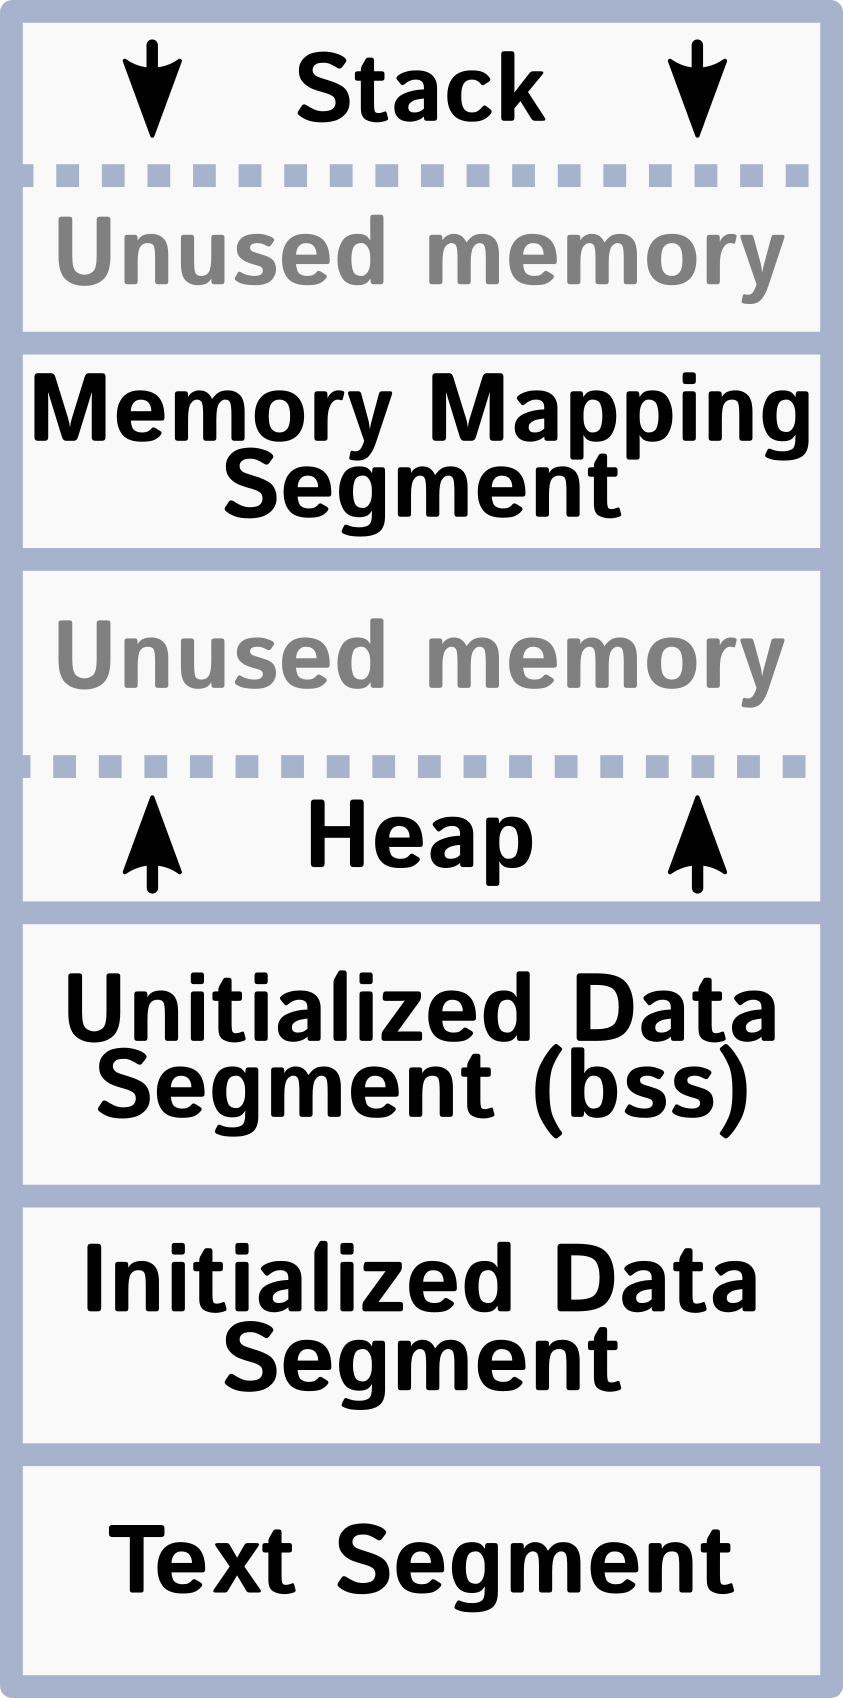
\includegraphics[width=.40\textwidth]{memory_segment} 
  \caption{Segmento de memória}
  \label{fig:memory_segment} 
\end{figure}

A Figura~\ref{fig:memory_segment} ilustra seis segmentos de memória diferentes
representando o leioute típico de um processo após sua criação (essa estrutura
pode variar a depender do SO e do compilador utilizado). O \boldAndIndex{segmento de texto} (\emph{text segment}) representa a região da
memória que mantém a cópia em memória do código executável (compartilhável e
apenas para leitura). O \boldAndIndex{segmento de dados inicializados}
(\emph{initialized data segment}) e o \boldAndIndex{segmento de dados não
inicializados} (\emph{uninitialized data segment})\footnote{O segmento de dados
não inicializável também é comumente conhecido como \emph{block started by
symbol (BSS)} por causa de um antigo operador usado pelos montadores
\citep{gdb}.} são responsáveis pelas variáveis estáticas. O
\boldAndIndex{segmento de mapeamento de memória} (\emph{memory mapping
segment}) é a região na qual o SO mapeia arquivos diretamente na memória (p.ex.,
bibliotecas dinâmicas ou arquivos especificados pelo programador). O
\boldAndIndex{segmento de pilha} (\emph{stack segment}) compreende os dados
usados pelo programa durante a execução, como por exemplo, valores de
parâmetros de função, endereços de retorno e variáveis locais (dados
temporários) \citep{silberschatz}. Por fim, o \boldAndIndex{segmento do monte (\emph{heap segment}}
mantém a memória dinamicamente alocada durante a execução do programa; repare
que a pilha e o \emph{heap} crescem em direções opostadas da memória.

O primeiro passo realizado pelo SO quando ele lê o arquivo executável é processar o \emph{header}, obtendo as informações sobre o tamanho dos segmentos de
texto e dados e criando um novo espaço de endereçamento (\emph{address space}).
O próximo passo consiste em alocar a memória inicialmente necessária e copiar
toda a região de código e dados lidas do arquivo binário do programa executável ou bibliotecas para essa memória
recém alocada. Em seguida, é feita a inicialização da PCB (descrita mais adiante)
e os devidos ajustes no \emph{stack pointer}\footnote{Um \emph{stack pointer} é
um registrador que armazena o endereço do último acesso feito pelo programa
para à pilha.} e no \emph{program counter} (PC), que é ajustado para a
o ponto de início do programa, por exemplo, a função \texttt{main} em um programa na linguagem C~\citep{patterson}. Por fim, quando o SO termina
de inicializar todos os elementos necessários para que o processo possa
executar, ele insere o novo processo na fila do escalonador.

\begin{figure}[!h]
  \centering
  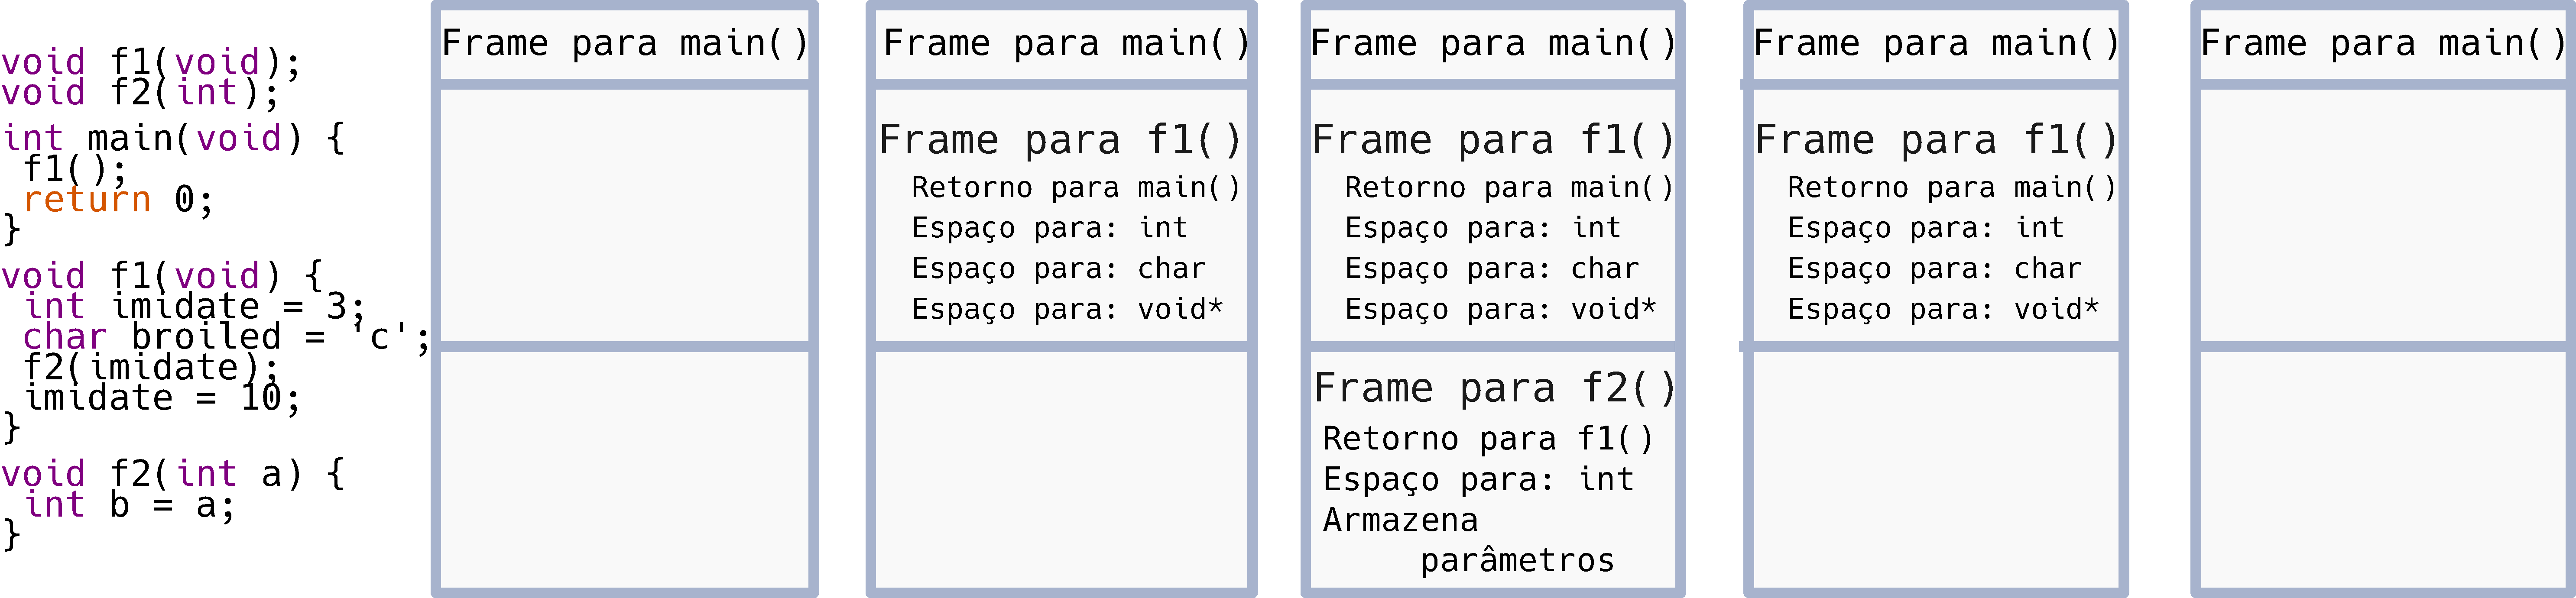
\includegraphics[width=\textwidth]{stack_frame}
	\caption[Alocação e desalocação de Stack frames considerando o padrão CDECL]{Alocação e desalocação de Stack frames considerando o padrão CDECL~\citep{patterson}}
  \label{fig:stack_frames} 
\end{figure}

% TODO: Fazer uma ponte melhor do PC com a execução

A pilha é organizada em uma coleção de \boldAndIndex{stack frames}, que
são estruturas de dados inseridas no topo da pilha e que contêm
informações como o endereço de retorno da função, argumentos recebidos,
variáveis locais, dentre outros. Toda vez que uma função é chamada, uma nova
estrutura de dados \emph{frame} é criada e preenchida com as informações
relacionadas à função.  A Figura~\ref{fig:stack_frames} ilustra a alocação e
desalocação de \textit{frames} em um simples programa \citep{gdb}. No começo,
só existe um \emph{stack frame} associado à função \texttt{main}. Conforme cada
função local é chamada, o SO aloca um novo \emph{stack frame}, que é inserido
logo após o \emph{frame} da função anterior. Esse procedimento permite que a
execução do processo ocorra de forma consistente, uma vez que basta desempilhar
o \emph{frame} para retomar ao contexto da função anterior. No fim da execução
da função, a execução retorna para o ponto na qual a função foi invocada e o
processo de preencher e esvaziar a pilha continua.

Todos os processos são descritos por meio de uma estrutura de dados chamada
\boldAndIndex{Process Control Block (PCB)}, responsável por manter informações
referentes ao estado do processo, \emph{program counter} (PC), registradores da
CPU, informações sobre escalonamento, dados sobre contas de usuários, estado de
operações de E/S, dentre outros \citep{silberschatz}.  Uma dos principais
motivos para a PCB existir é permitir a \textbf{troca de contexto}, o mecanismo
pelo qual processos se alternam no uso da CPU.  Por exemplo, se o usuário
possui vários processos executando concorrentemente, o SO deve alternar entre todos
eles para que cada um tenha a oportunidade de executar por um intervalo de
tempo. O SO realiza esse processo de troca em duas etapas: (1) salvamento do
estado atual do processo em sua PCB e (2) carregamento dos dados da PCB do
outro processo. A troca de contexto deve ser rápida para não prejudicar o desempenho das aplicações.

O conceito apresentado acima revela uma característica de isolamento associada
com a forma na qual os processos funcionam, promovendo segurança e
estabilidade.  Por outro lado, existem situações que demandam que os processos
cooperem entre si e, nesses casos, é possível notar algumas das desvantagens
inerentes da estratégia de processos atual. Para resolver parte desse problema,
algumas bibliotecas ou chamadas de sistema são fornecidas como interfaces para
coordenar a interação entre processos executando simultaneamente, oferecendo
mecanismos de \boldAndIndex{Comunicação entre processos}
(\boldAndIndex{Interprocess Communication}) ou simplesmente \boldAndIndex{IPC}.
Desenvolvedores podem utilizar IPC para compartilhar dados, melhorar o
desempenho das aplicações, refinar a modularidade da aplicação ou por alguma
questão de conveniência da sua aplicação. Os mecanismos de IPC têm três
limitações principais: elevam o consumo de memória, adicionam custos extras de
comunicação e apresentam uma certa complexidade para serem implementados. Essas
limitações são proibitivas em aplicações com grande demanda computacional.

Por muito tempo, buscou-se formas de elevar o desempenho das
aplicações por meio de melhorias no grau de paralelismo. No entanto, como
mencionado, o paralelismo tem seus próprios custos. Como resultado direto
do esforço em minimizá-los,
surgiu o conceito de um único processo com múltiplas \emph{threads}
compartilhando praticamente todos os elementos básicos de sua estrutura com exceção da
pilha e do PC. A Figura~\ref{fig:single_thread_multi_thread} mostra um
processo com uma \emph{thread} e outro com múltiplas \emph{threads}.

\begin{figure}[!h]
  \centering
  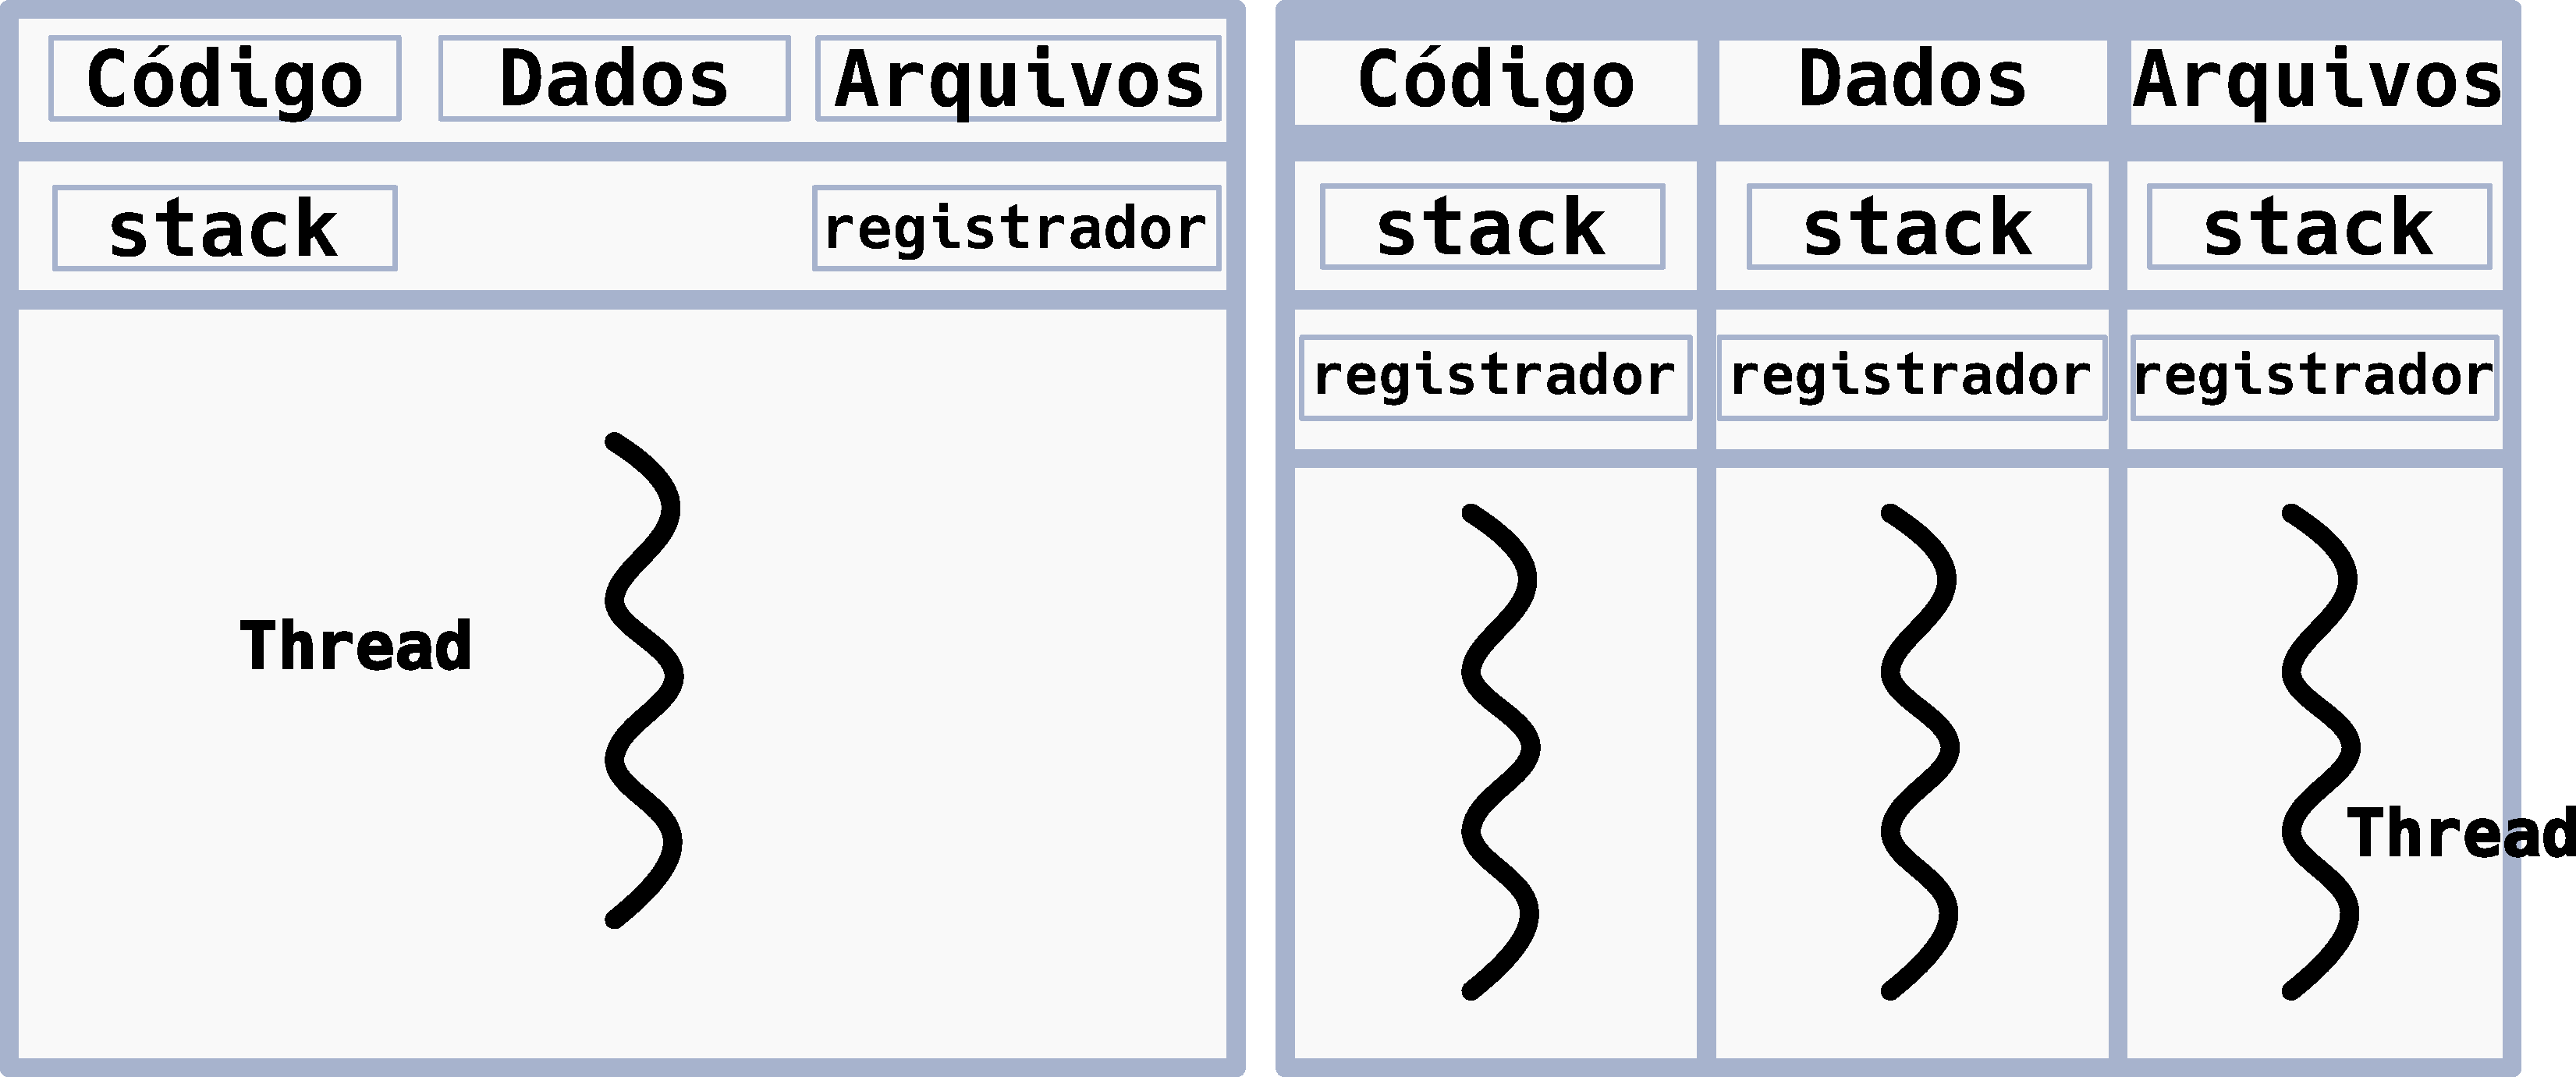
\includegraphics[width=.7\textwidth]{process_and_threads}
	\caption[Única thread e multi-thread.]{Única thread e multi-thread. Note o isolamento da pilha e dos registrador (PC)~\citep{silberschatz}}
  \label{fig:single_thread_multi_thread}
\end{figure}

Com o objetivo de ilustrar o comportamento descrito até agora sobre a execução
de múltiplas \emph{threads} em um mesmo processo, apresentamos um código
simples que tem por objetivo criar duas novas \emph{threads}, cada uma mostrando
uma mensagem diferente. O Código~\ref{lst:simplethreads} ilustra o
comportamento básico das \emph{threads} por meio de uma biblioteca chamada de
\emph{POSIX Thread Library (Pthread)}. A função
\texttt{thread\_kernel()} tem as operações que são executadas por cada nova
\emph{thread} criada na função principal. Note que \texttt{thread\_kernel()}
recebe um ponteiro genérico, converte-o para um tipo \texttt{char *} e
mostra o seu valor no final.

\begin{ruledcaption}{Exemplo simples de threads\label{lst:simplethreads}}
\lstinputlisting[
                 language=C,
                ]{code/simpleThread.c}
\end{ruledcaption}

A função \texttt{main()} declara duas variáveis do tipo \texttt{pthread\_t},
que são responsáveis por manter as informações referentes às \emph{threads}.
Adicionalmente, são declaradas duas \emph{strings} diferentes para serem
mostradas posteriormente dentro das \emph{threads} criadas de forma a
tornar claro o paralelismo. Quando o PC atinge a função
\texttt{pthread\_create()}, a biblioteca solicita ao SO a criação de uma nova
\emph{thread} que executa a função \texttt{thread\_kernel()} em paralelo. Em
seguida, \texttt{pthread\_create()} é chamada novamente e cria uma segunda
\emph{thread} de execução baseada na função \texttt{thread\_kernel()}, contudo,
com outra mensagem associada com ela. Note que nesse momento da execução, temos
três \emph{threads}: a primeira \emph{thread} criada durante a inicialização do
processo e outras duas \emph{threads} criadas por meio da função
\texttt{pthread\_create()}. O código termina com a função
\texttt{pthread\_join()}, que mantém a \emph{thread} principal esperando que as
duas \emph{threads} terminem a sua execução. Uma das possíveis saídas desse
programa é ilustrada na Figura~\ref{lst:simpleThreadOutput}. Ela mostra que as
duas \emph{threads} executam em paralelo, o que é evidenciado pela sequência não
determinística da saída: A diferença na sequência é explicada pela variação
imposta pelo escalonador.

\begin{ruledcaption}{Saída do exemplo de threads\label{lst:simpleThreadOutput}}
\lstinputlisting[
    language=bash,
    ] {code/output.sh}
\end{ruledcaption}

Vamos analisar com um pouco mais de detalhes como o SO trata o
Código~\ref{lst:simplethreads} durante a sua execução. A
Figura~\ref{fig:stack_threads} ilustra o que acontece internamente quando novas
\emph{threads} são criadas. Como esperado, o segmento de texto e dados são
compartilhados entre as \emph{threads}, como ilustrado na parte inferior da
figura. A principal mudança na organização de memória pode ser observada no
segmento da pilha, pois toda vez que uma nova \emph{thread} é criada um
novo segmento de pilha é gerado (a Figura~\ref{fig:stack_threads} mostra
que a pilha é preenchida aos poucos); a independência entre
\emph{threads} é assegurada pelas múltiplas pilha isoladas. Cada \emph{thread}
tem seu próprio \emph{stack pointer} e demais registradores; toda vez que a
\emph{thread} em execução muda, o \emph{stack pointer} e os registradores são
atualizados. Repare que o uso de \emph{threads} melhora o desempenho uma vez
que reduz os impactos na memória cache (detalharemos mais sobre esse aspectos
nas próximas seções).

\begin{figure}[!h]
  \centering
  \includegraphics[width=.80\textwidth]{theads_and_stack} 
	\caption[Um processo com uma thread e um processo com três threads]{Um processo com uma thread (esquerda) e um processo com três threads (direita)}
  \label{fig:stack_threads} 
\end{figure}

\section{Gerenciamento da Memória Relacionada aos Processos}

Fazer com que a memória do sistema esteja disponível e utilizável para uma
aplicação é uma das principais responsabilidade de um SO de propósito geral. A
maioria dos SOs modernos oferece a ilusão de que toda a memória está acessível
para cada processo, o que é possível graças ao desacoplamento entre a memória
física e como o processo a vê. Processos só veem o \emph{Virtual Address Space
(VAS)} que, por sua vez, é mapeado pelo SO (com auxílio de hardware) para a
memória física, garantindo um bom isolamento entre processos. Além da ilusão de
que a memória está inteiramente disponível para cada processo, esse mecanismo
também permite que (1) a memória alocada para um dado processo não seja
necessariamente contígua, permitindo uma melhor utilização dos recursos, (2)
trechos de memória iguais em processos diferentes, como o segmento de texto,
possam ser compartilhados, economizando espaço, e (3) seja possível liberar
memória temporariamente, associando um trecho de memória virtual com uma área
de disco.

%Para manipular VASes e oferecê-las para as aplicações do usuário, os SOs adotam
%um modelo de memória específico.  Atualmente, a maioria dos SOs de produção e
%hardware suportam amplamente o modelo de gerenciamento de páginas. Esse modelo
%separa a espaço de endereçamento virtual e físico para cada processo em um
%conjunto de páginas, cada uma correspondente a um pequeno intervalo contíguo de
%endereços de tamanho fixo, identificadas pelo endereço de início e com
%permissões específicas.

% TODO: Relocar essa informação? Apagar? Eis a questão
% O modelo de paginação oferece algumas vantagens: controle das permissões no
% nível da página, mecanismos de compartilhamento, rápida verificação de
% proteção, notificações acuradas sobre violações e a possibilidade de mapear
% memória em disco.

% TODO: Introduzir brevemente o modelo de segmentação? NELSON: Sim, uma frase, mais ou menos do mesmo tamanho da que está aí explicando o modelo de paginação

%\subsection{Endereços Lógicos, Físicos e Paginação}

% TODO:  Nessa seção, não temos a intenção de discutir profundamente os mecanismos presentes 
% TODO: O meu objetivo nesse primeiro parágrafo era introduzir a questão dos
% endereçamentos, por isso fiz uma pequena volta sobre a questão do binário. Será que da para encurtar? Como?

Quando o software começa a sua execução, significa que a CPU está executando as
instruções descritas no binário, dentre elas as tentativas de acesso a certos
endereços na memória. Todo endereço utilizado pela CPU nesse contexto recebe o
nome de \boldAndIndex{endereço virtual} ou \boldAndIndex{endereço lógico}; por
sua vez, o conjunto desses endereços recebe o nome de \boldAndIndex{espaço de
endereçamento virtual (Virtual Address Space)} ou simplesmente \boldAndIndex{VAS}. Esses
endereços não são válidos da perspectiva da memória física, i.e., são apenas
endereços usados pela aplicação mas que não correspondem ao endereço real dessa
memória física. Os endereços reais da memória são chamados de
\boldAndIndex{endereços físicos} e o conjunto de todos os endereços da memória
são chamados de \boldAndIndex{espaço de endereçamento físico}. Agora você deve
estar se perguntando: qual a relação entre esses dois tipos de endereços? Eis
que surge um terceiro elemento entre elas, a \boldAndIndex{Memory-Management
Unit (MMU)}. Veja a Figura~\ref{fig:mmu} ilustrando como a MMU se interpõe
entre o endereço lógico e o físico.

\begin{figure}[!h]
  \centering
  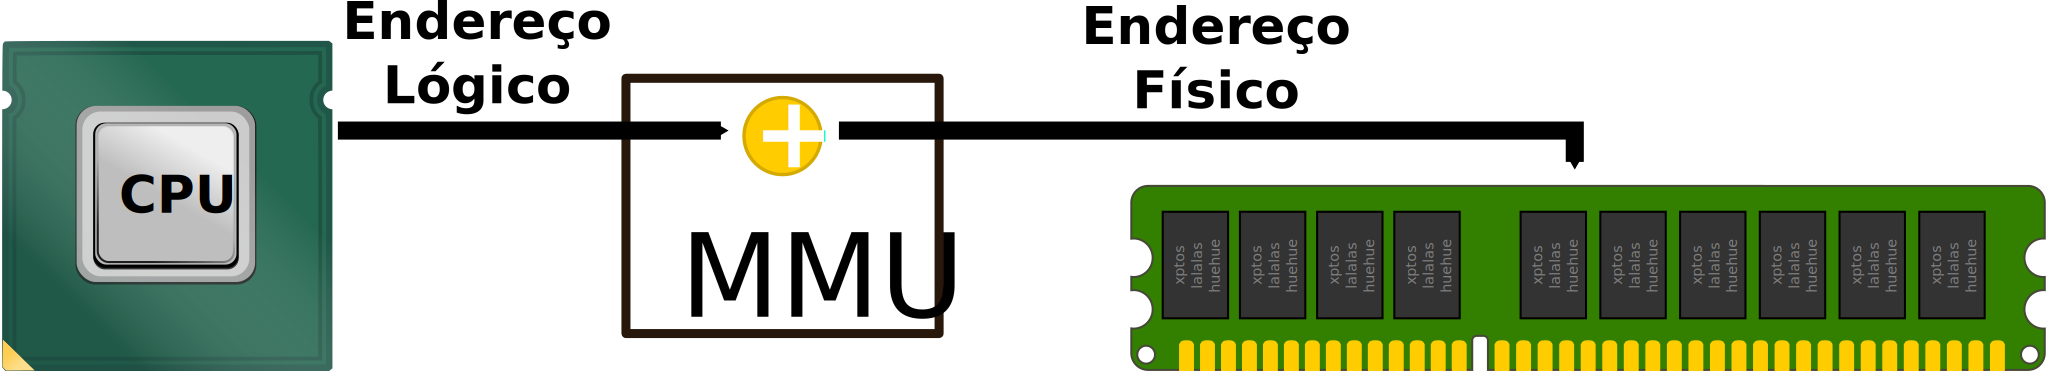
\includegraphics[width=\textwidth]{mmu} 
  \caption{Do endereço lógico ao físico com o auxílio da MMU}
  \label{fig:mmu}
\end{figure}

A MMU é um hardware usado para fazer o mapeamento do endereço virtual para o
endereço físico em tempo de execução. A Figura~\ref{fig:mmu} mostra a CPU
gerando um endereço lógico que é imediatamente entregue para a MMU. Esta
converte o endereço recebido em um endereço físico e procede com o acesso à
memória.

Qual o tamanho máximo da memória de um sistema?  No caso da memória virtual, o
endereçamento começa em 0 e vai até um valor máximo definido em um conjunto de
bits chamado de \boldAndIndex{virtual bits}. Durante muito tempo, o padrão
adotado para o \emph{virtual bits} era de 32 bits, gerando um limite superior
de endereçamento de 4 GiB; hoje em dia é relativamente comum encontrar CPUs que
fornecem 48 bits, produzindo uma VAS de 256 TiB. Na prática, isso significa
que um software executado em um SO moderno tem a ilusão de que pode acessar
todos os endereços fornecidos pela VAS. Por enquanto, sabemos que isso não é
verdade, pois dificilmente conseguimos fornecer tanta memória. Por esse motivo,
e como ilustrado na Figura~\ref{fig:vas_pas}, notamos que o endereço virtual
pode ser várias vezes maior do que o endereço físico. Além disso, repare que a
memória física deve ser compartilhada entre vários processos em execução no SO
(todos eles acreditam que tem toda a memória disponível).

\begin{figure}[!h]
  \centering
  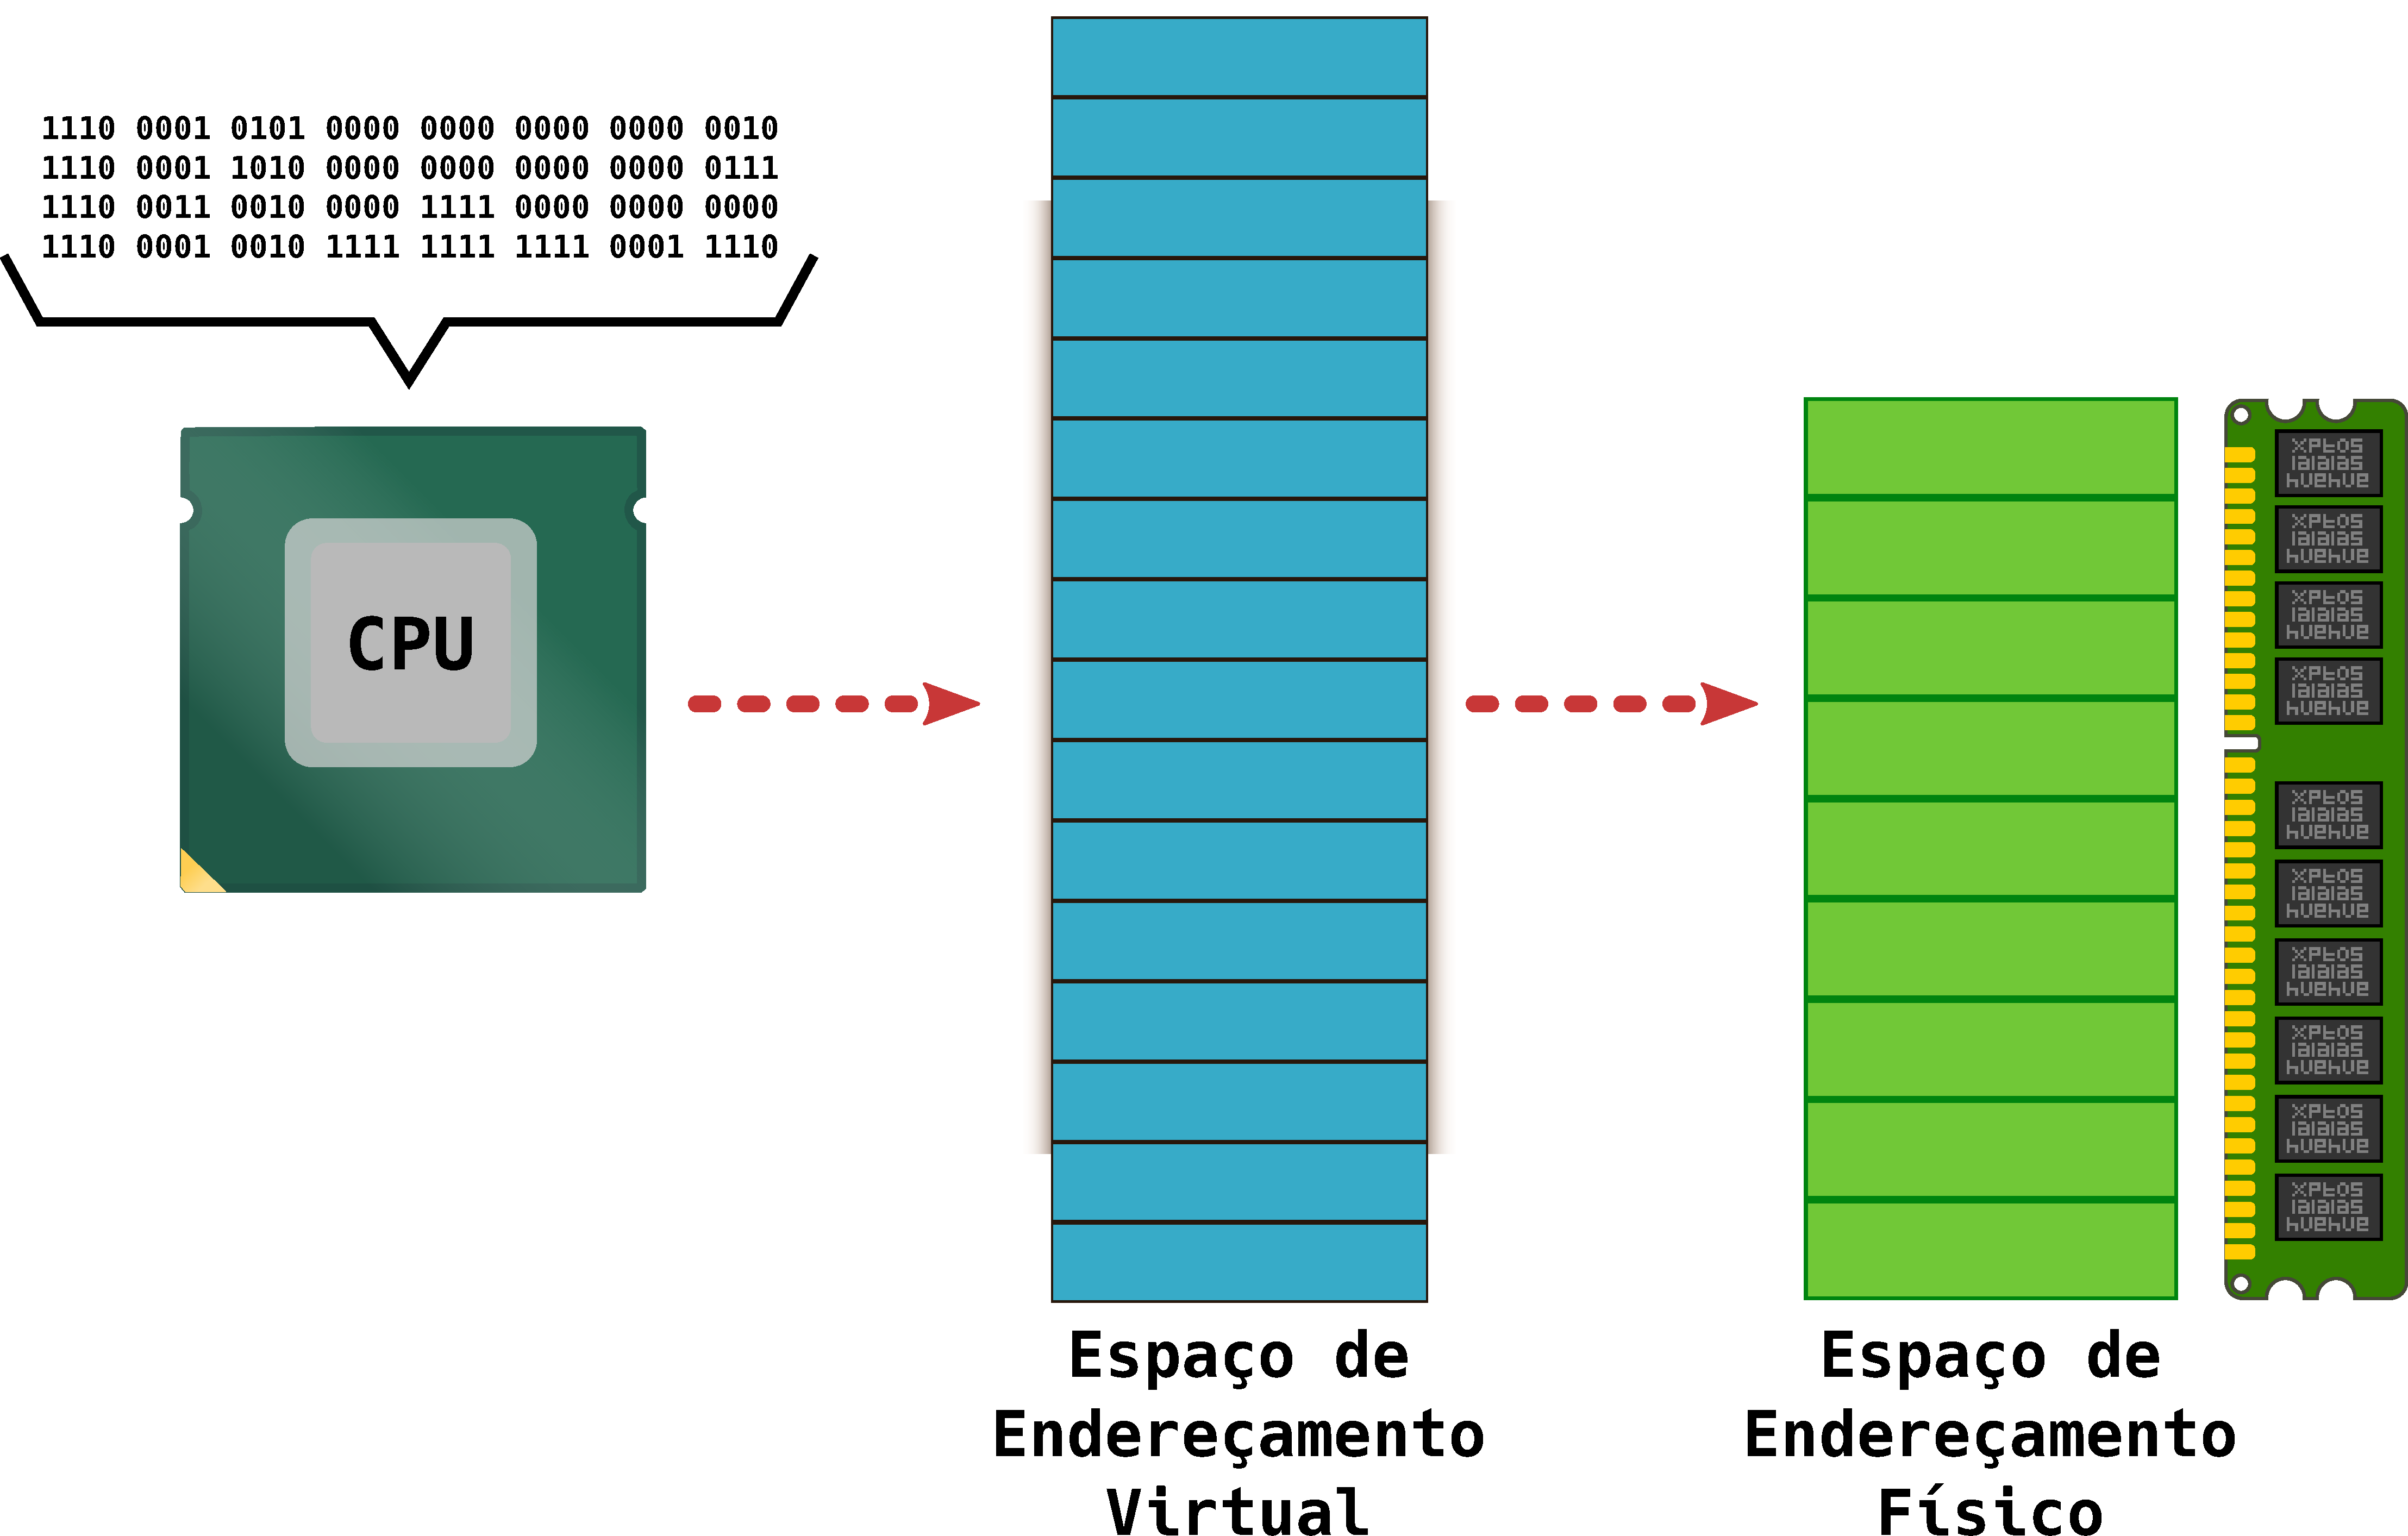
\includegraphics[width=.5\textwidth]{virtual_vs_fisico} 
  \caption{Espaço de endereçamento virtual vs. físico}
  \label{fig:vas_pas}
\end{figure}

%TODO: AQUI VEM O GANCHO

Não obstante, como fazer para traduzir um endereço VAS para um endereço físico?
Não é viável ter uma tabela de tradução byte-a-byte (ela ocuparia toda a
memória) nem supor que a memória de um processo é contígua. A solução é
dividir a memória em blocos e manter, para cada processo, uma tabela mapeando
cada bloco dentro do VAS para um bloco correspondente na memória física. Há
duas estratégias comuns para isso: o modelo de paginação e o modelo de
segmentação.

\subsection{O Modelo de Paginação}
\label{sec:modelopaginacao}

Para implementar o modelo de páginação, é preciso dividir o espaço de
endereçamento virtual em \boldAndIndex{páginas} e o físico em
\boldAndIndex{frames}. Uma vez que ambos os espaços de endereçamentos são
subdivididos, é necessário ter um mecanismo para saber o que está presente ou
não na memória. Para ter uma visão de como todo o modelo de paginação funciona,
veja a Figura~\ref{fig:paginacao}.

\begin{figure}[!h]
  \centering
  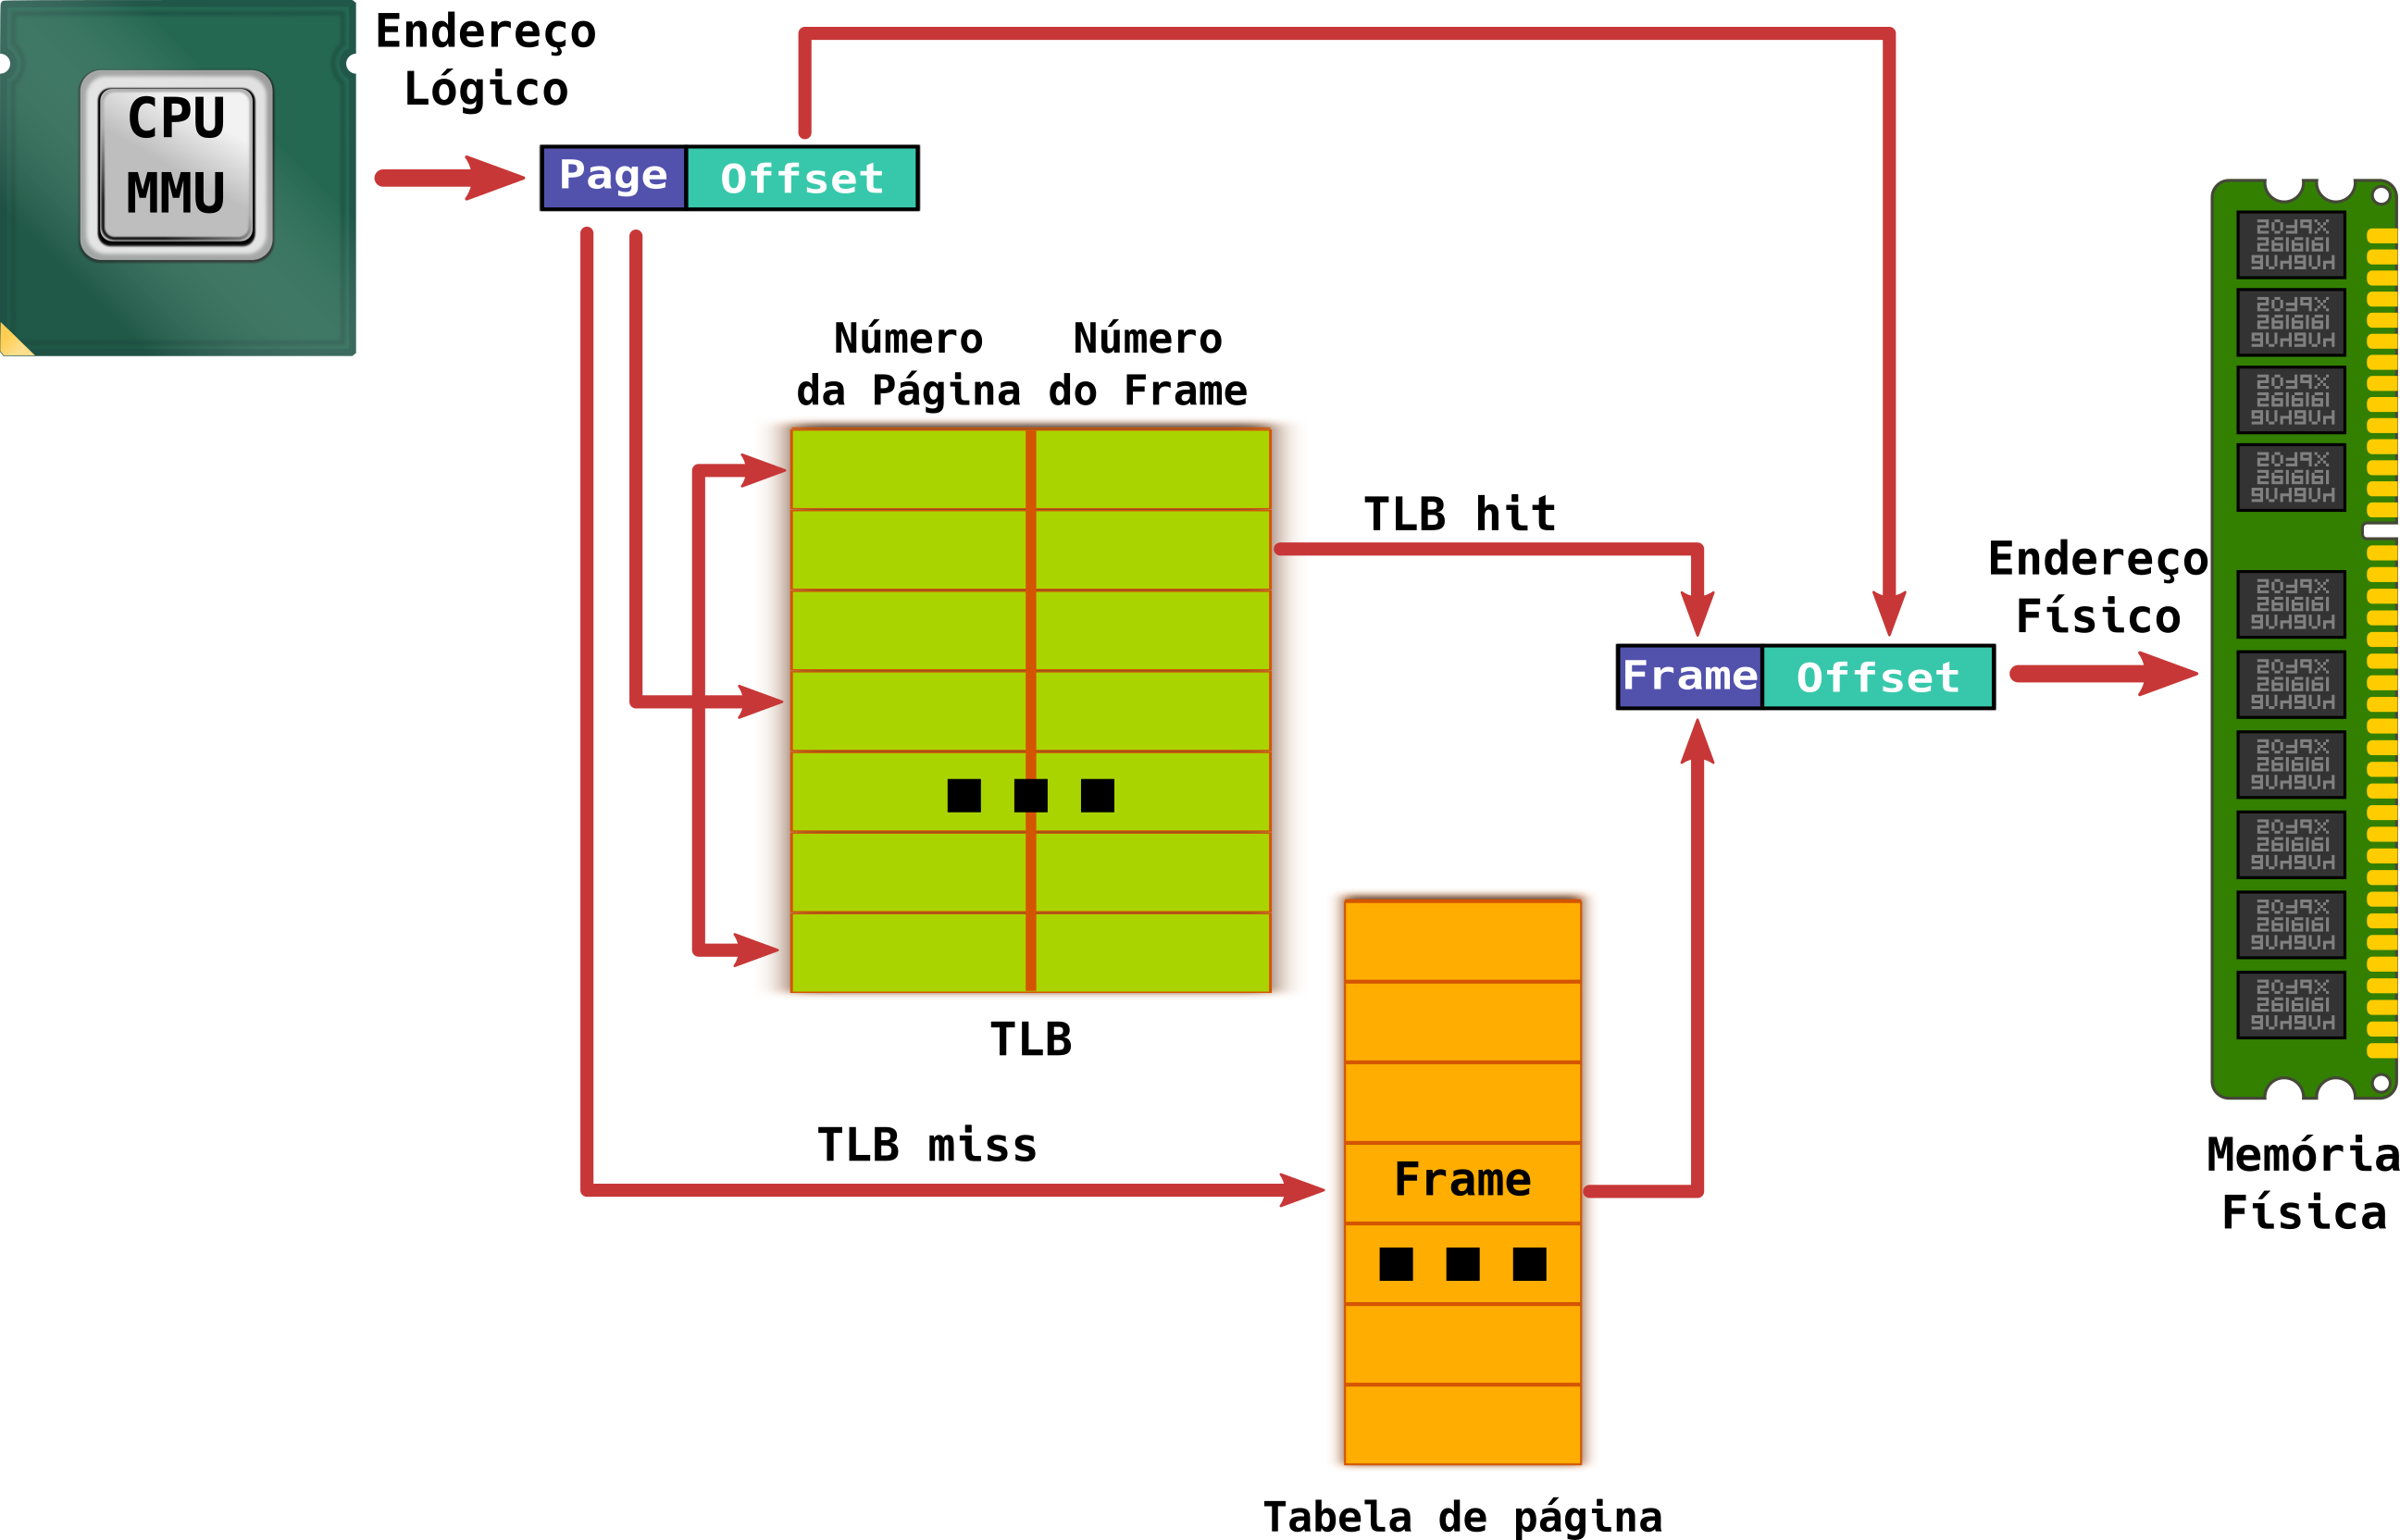
\includegraphics[width=0.8\textwidth]{paginacao} 
	\caption[Os elementos básicos presentes no modelo de paginação.]{Os elementos básicos presentes no modelo de paginação. Note que a busca na TLB e na tabela de página ocorre em paralelo}
  \label{fig:paginacao}
\end{figure}

Na Figura~\ref{fig:paginacao} observamos que a CPU gera um endereço lógico,
subdividido em duas partes: \textit{page} e um \textit{offset}. O \emph{page}
comporta-se como um índice corresponde a uma entrada em uma estrutura de dados
chamada \boldAndIndex{tabela de paginação}. Essa tabela faz parte da abstração
de processos e tem uma entrada especificada na PCB, ou seja, todo processo
possui uma tabela associada a si. Cada entrada na tabela corresponde ao
endereço de início de um \emph{frame} na memória associado ao processo.  Para
ilustrar melhor esse conceito, imagine um programa que aloca espaço na memória.
Em termos práticos, o SO cria uma nova entrada na tabela e retorna o endereço
virtual para a aplicação.  Depois que o valor referente ao índice é recuperado
a MMU soma o \textit{offset} da segunda parte do endereço virtual e, finalmente,
o acesso a memória física ocorre.

\begin{figure}[!h]
  \centering
  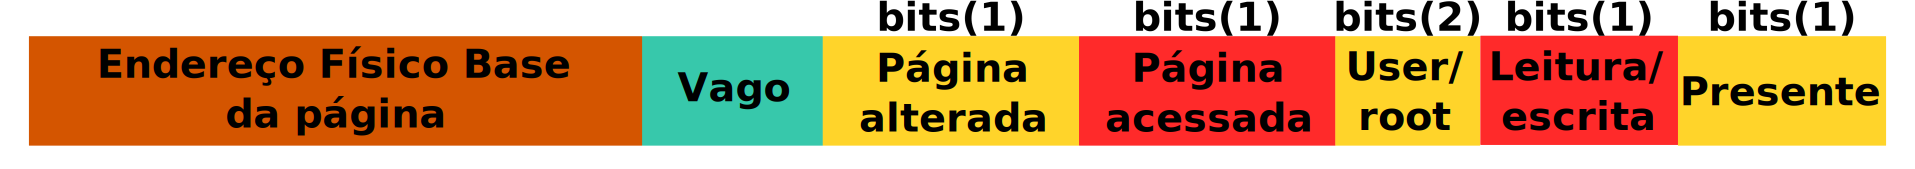
\includegraphics[width=\textwidth]{pte}
  \caption{Entrada da tabela de páginas}
  \label{fig:pte}
\end{figure}

Toda vez que um acesso à memória é feito, a tabela de páginas do processo é
consultada. Cada entrada dessa tabela é descrita por uma série de metadados que
descreve a região de memória e recebe o nome de \boldAndIndex{entrada da tabela
de páginas} (\textit{Page Table Entry}) ou simplesmente PTE. A
Figura~\ref{fig:pte} ilustra como a entrada pode ser representada\footnote{Cada
arquitetura implementa a PTE à sua maneira.}. Sem entrar em detalhes referentes
aos campos (a figura é autoexplicativa), podemos concluir que uma página
virtual é a unidade mínima de proteção da memória, por que todos os bytes dela
compartilham os bits User/Root e Leitura/Escrita.

\begin{figure}[!h]
  \centering
  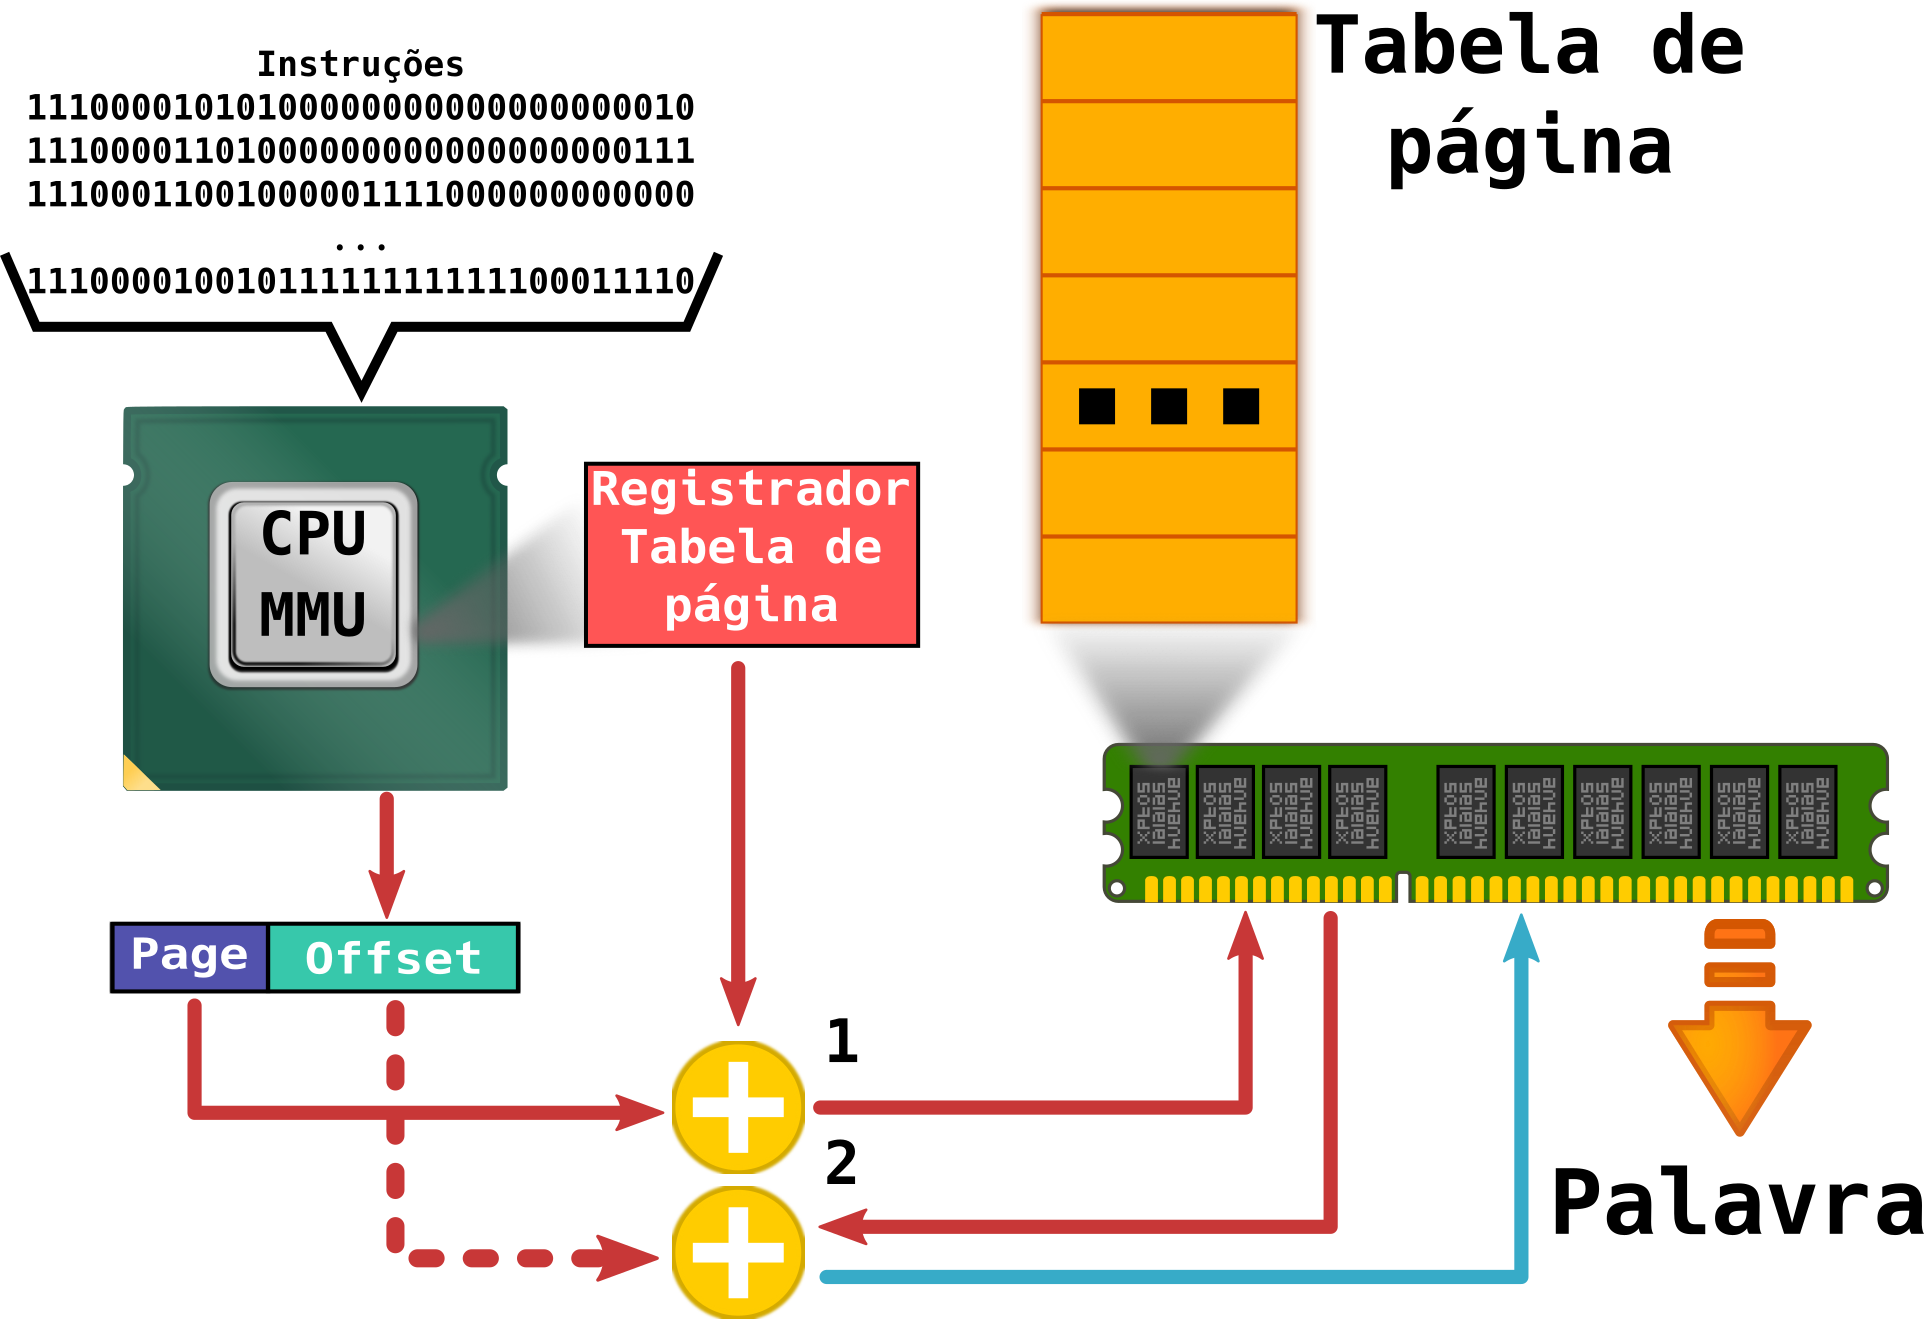
\includegraphics[width=0.8\textwidth]{paginacao_passos} 
	\caption[Passos do acesso a memória usando o modelo de paginação.]{Passos do acesso a memória usando o modelo de paginação. A figura ilustra o caso simples na qual pelo menos dois acessos a memória são necessários}
  \label{fig:passos_paginacao}
\end{figure}


A Figura~\ref{fig:passos_paginacao} exemplifica o processo completo de
converter um endereço virtual até o acesso na memória física. Repare que são
necessários vários acessos à memória para construir o endereço físico e
finalmente conseguir acessar a palavra de dados, o que faz com que essa técnica
não seja eficiente.  Nesse sentido, existe um mecanismo que busca reduzir esses
acessos por meio de uma tabela chamada de \boldAndIndex{translation look-aside
buffer (TLB)}. Essa tabela salva o último acesso (coluna e valor) feito à
tabela de páginas evitando que a memória seja consultada inúmeras vezes. Na
Figura~\ref{fig:paginacao}, é possível ver a TLB sendo usada para acelerar o
acesso aos dados: se uma consulta for encontrada na TLB, ocorre o chamado
\boldAndIndex{acerto na TLB (TLB hit)}; do contrário, \boldAndIndex{falta na
TLB (TLB miss)}. Note que a busca na memória sempre é feita, o que significa
que, no pior caso (\emph{TLB miss}), a busca na memória já foi iniciada. Além
disso, o mecanismo de paginação facilita a operação de realizar o
compartilhamento de dados entre os processos; o SO orquestra um conjunto de
páginas com a mesma visibilidade (indicada pelo programa no espaço de usuário)
para ser compartilhado entre processos.

\subsection{Modelo de Segmentação}
\label{sec:segmentacao}

Além do mecanismo de gerenciamento de memória fornecido pela paginação, também
existe uma alternativa chamada de \boldAndIndex{segmentação}. Esse modelo
decompõe a memória referente ao programa em segmentos de acordo com as suas
seções; por exemplo, uma área para o \textit{text}, outra para os dados,
pilha, etc. Os tamanhos de cada segmento podem ser variáveis, o que
leva a uma visão bidimensional da memória uma vez que os endereços passam a ser
construídos como uma tupla: \texttt{<número do segmento, offset>}
\citep{silberschatz}. Apesar dessa visão bidimensional, a memória continua
sendo linear e, por isso, é necessário converter os endereços.

O modelo de segmentação depende de um elemento fundamental chamado
\boldAndIndex{tabela de segmentos}. A tabela de segmentos é o elemento central
para a conversão de um endereço lógico em um endereço físico, ela mantém o
mapeamento das referências para o começo de cada segmento do programa. Cada
entrada dessa tabela é dividida em dois pedaços chamados de limite e base. O
limite é um componente com duas responsabilidades, (1) ele é o índice de um
elemento na tabela e (2) o seu valor indica o tamanho máximo do segmento. Por
sua vez, o limite está associado a um segundo valor chamado de endereço base
(ou simplesmente base) que representa o início do segmento na memória física.

A Figura~\ref{fig:segmentacao} mostra como a segmentação funciona com o suporte
de hardware. Repare que o endereço lógico utilizado pela CPU é dividido em duas
partes; a primeira parte do endereço corresponde ao limite e a segunda a um
\emph{offset}. Como ilustrado na figura, o valor do limite é utilizado para
acessar a tabela de segmentos e recuperar o valor base. O limite é o tamanho
máximo do segmento e é usado para verificar se o \emph{offset} passado é
valido. Se a verificação do limite for válida, então o endereço base é lido e
usado em conjunto com o \emph{offset} para gerar o endereço físico.

\begin{figure}[!h]
  \centering
  \includegraphics[width=.80\textwidth]{segmentacao} 
	\caption[Comportamento do modelo de segmentação.]{Comportamento do modelo de segmentação. Note que a tabela de segmento é acessada para obter o valor base e esse é sempre verificado para evitar acessos indevidos a outras regiões da memória}
  \label{fig:segmentacao} 
\end{figure}

Tanto o modelo de segmentação quanto o de paginação têm suporte de hardware.
Tradicionalmente o Microsoft Windows fez uso do modelo de segmentação, enquanto
o MacOS e o GNU/Linux usam a paginação. Como a CPU costuma dar suporte para
ambos os esquemas, os SOs podem utilizar esses mecanismos para executar
aplicações de outros SOs. Por exemplo, o
Wine\footnote{\url{https://www.winehq.org/}} executa aplicações Windows no
Linux utilizando parte dos recursos de segmentação fornecidos pela CPU.

\subsection{Proteção da memória}
\label{sec:outros_mecanismos_memoria}

A Seção~\ref{sec:modelopaginacao} descreveu a forma como o mecanismo de
paginação funciona, em especial, apresentamos uma ilustração de uma PTE na
Figura~\ref{fig:pte}. A PTE define um certo nível de proteção da memória uma
vez que temos bits que servem para verificar se a página é acessível ou não
pelo programa. Contudo, as CPUs modernas estão evoluindo de forma a fornecer
novos recursos de controle de acesso à memória. Em especial as CPUs Intel e ARM
já oferecem uma funcionalidade chamada de \boldAndIndex{Chave de Proteção da
Memória} (\emph{Memory Protection Key}).

Essa nova funcionalidade permite que um processo tenha mais opções de controle
de acesso a memória, i.e., o processo pode restringir o acesso dele mesmo a
certas regiões da memória. Para possibilitar que tal mecanismo seja
implementado, as CPUs passaram a oferecer um mecanismo que faz uso de quatro
bits da PTE que não eram utilizados. A Figura~\ref{fig:ptedominio} ilustra uma
PTE utilizando esses bits, em última instancia esse é mais um recurso atrelado
à tabela de tradução. No total, esses 4 bits representam um conjunto de 16
possíveis domínios de acesso. 

\begin{figure}[!h]
  \centering
  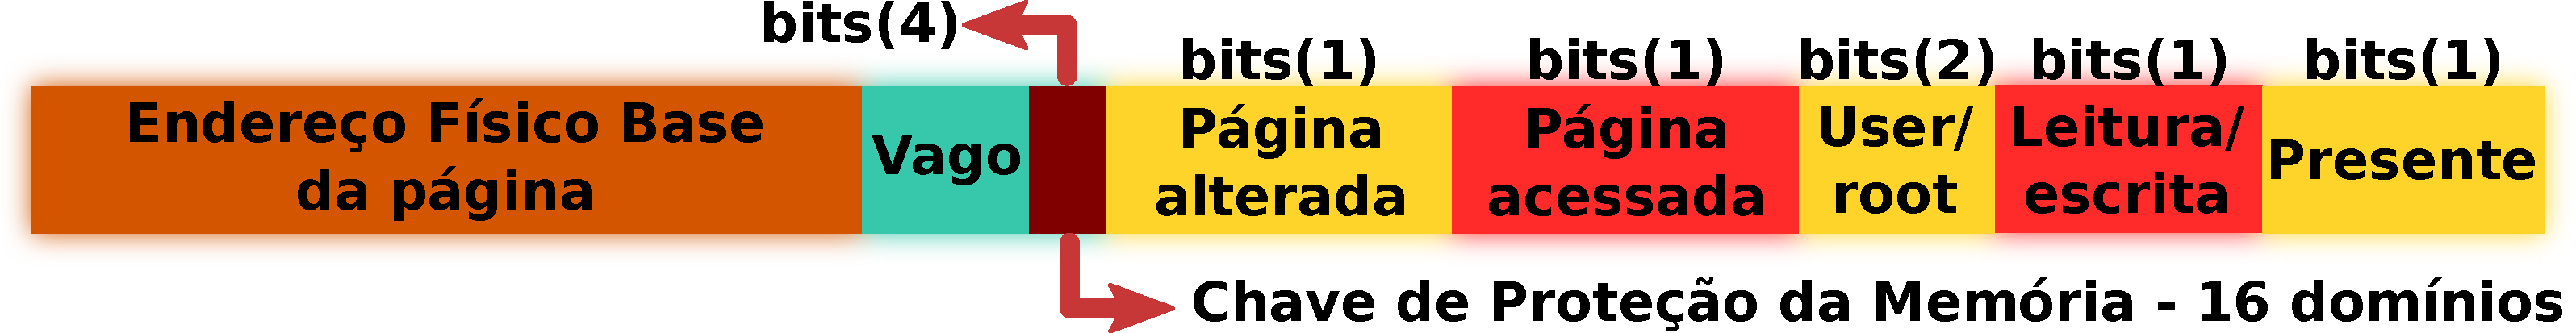
\includegraphics[width=.80\textwidth]{pte_domain} 
  \caption{Ilustração de uma entrada da tabela de páginas utilizando novos bits}
  \label{fig:ptedominio} 
\end{figure}

Cada região de memória definida na tabela de tradução é controlada por um dos
16 domínios existentes~\citep{armdeveloperguide}.  O aspecto mais interessante
em se utilizar domínios está nos possíveis comportamentos que eles apresentam
caso ocorra alguma tentativa de acesso à memória, dentre eles: o acesso pode
ser permitido se o conjunto de permissões presentes na tabela permitir e gerar
falta de domínio. A MMU procede com algumas verificações, que consistem em três
passos:

\begin{enumerate}
  \item A MMU verifica o número do domínio encontrado na tabela de tradução;
  \item Com base no número obtido do passo anterior, a MMU verifica a permissão
        de acesso no registrador de controle de acesso;
  \item De acordo com o valor encontrado no registrador de domínio de acesso, a
        MMU pode tomar as seguintes decisões: permitir o acesso, bloquear o
        acesso e verificar a permissão de acesso em uma tabela de tradução.
\end{enumerate}

Assim, o SO precisa decidir, para cada aplicação se o acesso à diferentes áreas
de memória deve ser permitido ou negado.  Além disso, o SO pode mudar
permissões de acesso para um grande número de regiões simultaneamente. Note que o
mecanismo de domínios é um recurso adicional ao tradicional modelo de controle
da memória adotado pelos SOs, ou seja, é um recurso não fundamental mas que
oferece novos recursos aos desenvolvedores.

\subsection{Exemplo Prático Usando o GNU/Linux}
\label{sec:visao_pratica_mem}

Nesta seção, revisitamos e expandimos alguns dos conceitos discutidos da
perspectiva do Linux, já que a maioria dos trabalhos analisados faz uso
de SOs baseados nele. Iniciamos a nossa análise por um fato interessante sobre VAS no Linux em uma
arquitetura x86: uma vez que a VAS é habilitada, todo sistema é afetado,
incluindo o próprio kernel. Por esse motivo, uma porção da VAS é reservada para
o Linux; contudo, ela recebe um tratamento especial, uma vez que o acesso a ela é
restrito e o kernel está presente na memória física. Por outro lado, as VASes dos
processos comportam-se como o esperado, ou seja, são movidas constantemente de
acordo com a troca de contexto e podem ser acessadas pela aplicação. A
Figura~\ref{fig:vas_contexto} busca ilustrar o mapeamento da VAS levando-se em
consideração o espaço reservado para o Kernel (destacado no topo da figura) e os
processos. O lado esquerdo da figura mostra de forma genérica como o Kernel e
uma aplicação coexistem na memória. Repare que o processo tem todos os seus
segmentos alocados da memória e a ilusão de que tem total domínio sobre ela,
i.e., comporta-se como descrito na Seção~\ref{sec:processos-e-threads}. Por
outro lado, o processo não tem acesso ao intervalo de endereços reservados
para o Kernel. Por fim, do lado direito da figura, é mostrado como a troca de
contexto ocorre entre dois processos; repare que a VAS dos processos são
substituídas mas o kernel permanece constante.

\begin{figure}[!h]
  \centering
  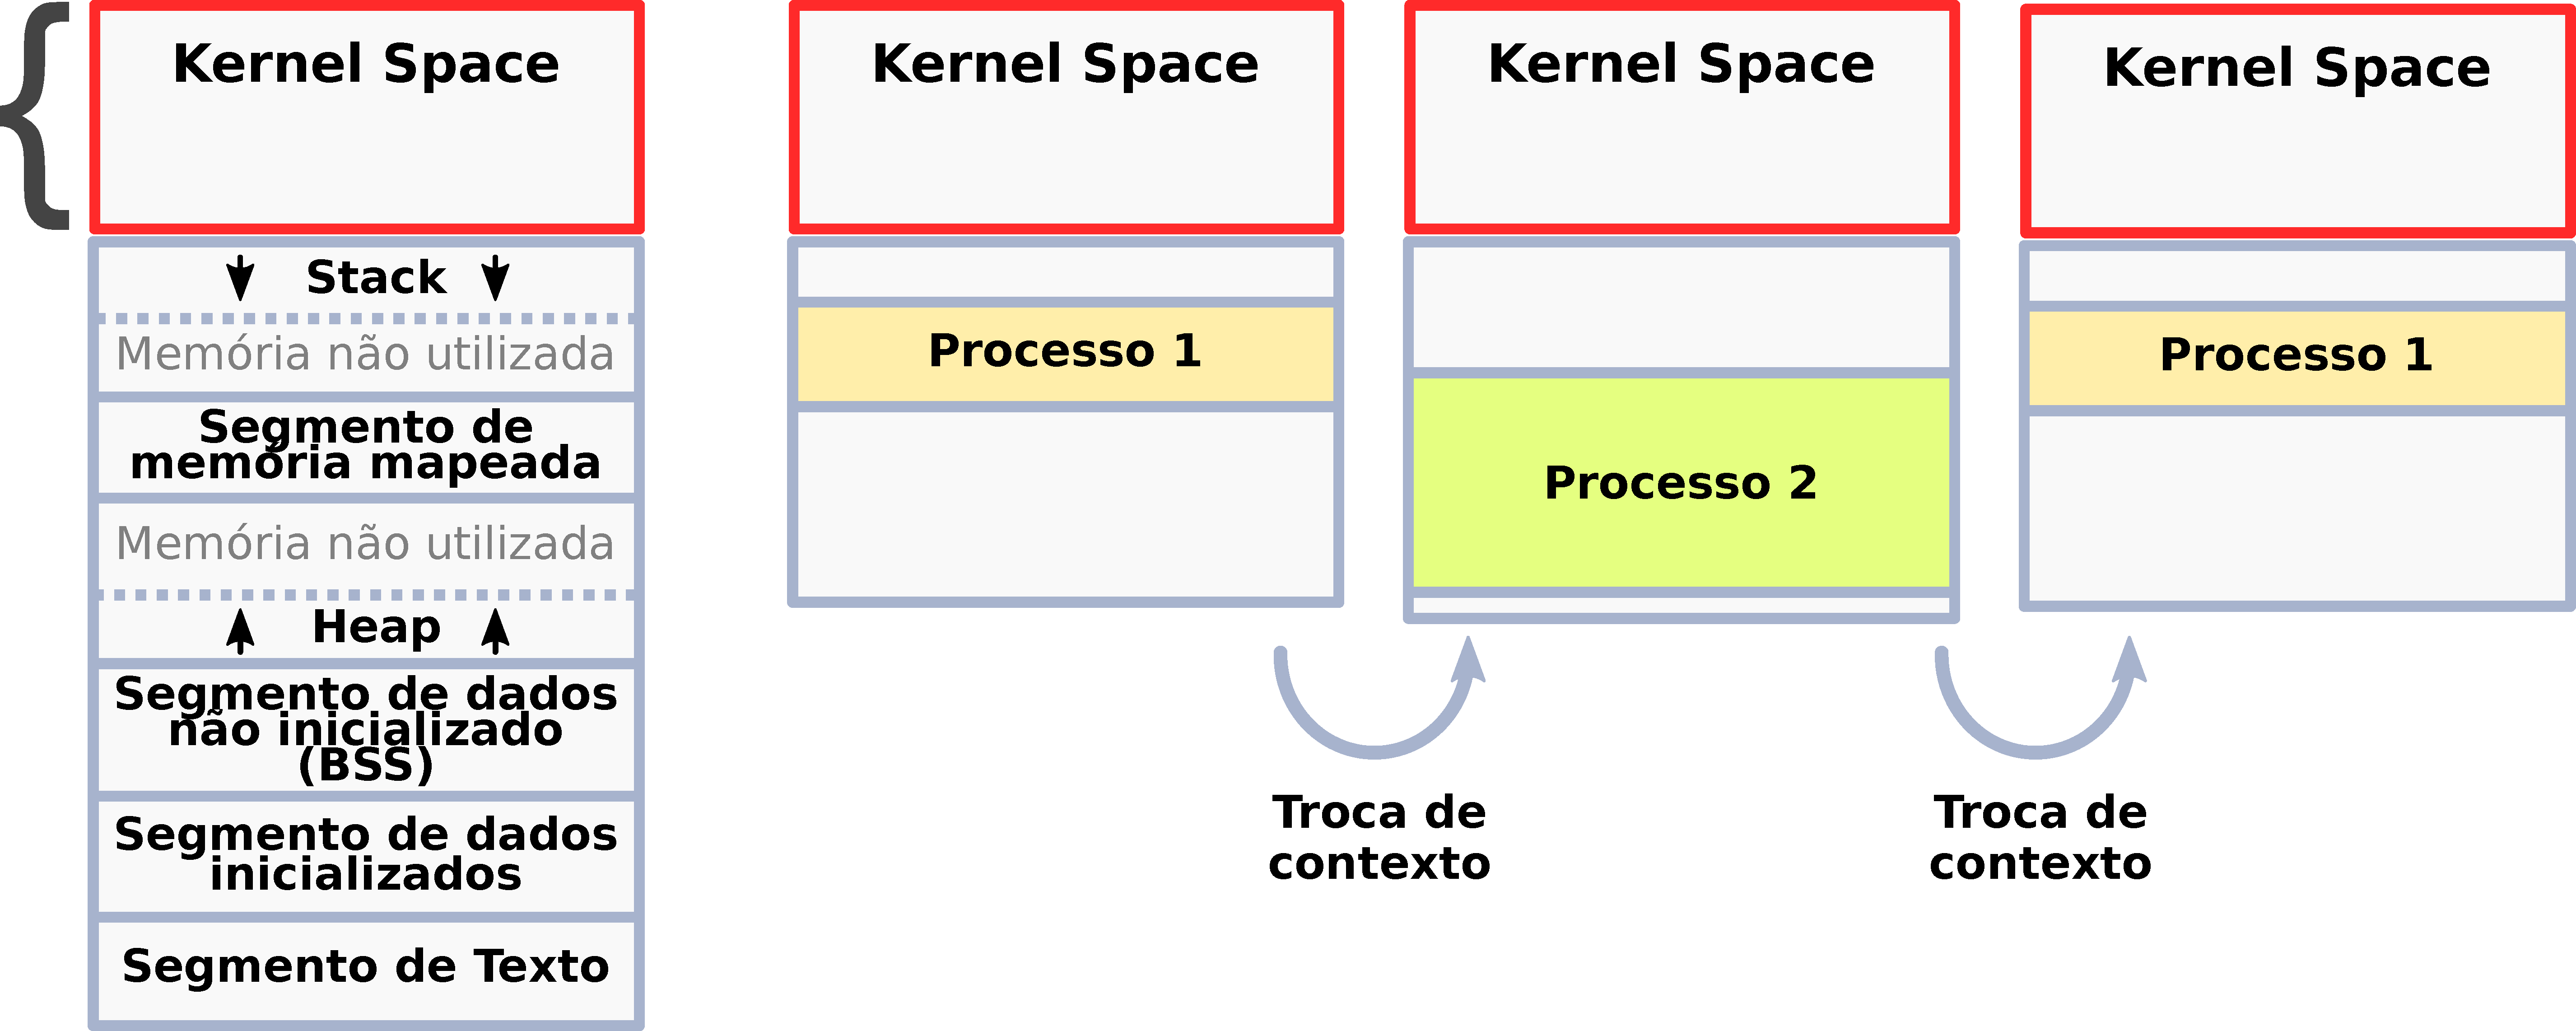
\includegraphics[width=\textwidth]{segmento_troca_contexto}
	\caption[VAS durante a troca de contexto]{VAS durante a troca de contexto~\citep{kernel_manage_mem}}
  \label{fig:vas_contexto}
\end{figure}

Note que, até esse momento, temos uma visão de uma sequência padrão para os
segmentos do processo descrita pela ordem: \emph{text}, \emph{dados
inicializados}, \emph{BSS}, \emph{heap}, \emph{mapeamento de memória} e
a pilha. Esse tipo de informação torna o sistema mais vulnerável, uma vez
que um atacante que conheça tal sequência terá uma forma de encontrar dados na
memória explorando uma eventual falha de segurança. Como uma resposta a essa situação,
o Kernel implementa uma série de mecanismos de embaralhamento
conhecidos como ASLR\footnote{\url{https://lwn.net/Articles/330866/}}, KASLR e
KARL~\citep{kaslr}. Dentre as áreas a que o Linux aplica a aleatorização,
destacam-se os segmentos dos processos. Portanto, toda vez que um processo é
inicializado o seu leioute na memória é embaralhado aleatoriamente, dificultando um eventual
ataque.

Ainda na Figura~\ref{fig:vas_contexto}, tenha em mente que o programa em
execução faz alocações na pilha durante a sua execução, como explicado
na Seção~\ref{sec:processos-e-threads}. No Linux, essa pilha começa
com um tamanho pré-definido (8 Mb) que normalmente é o suficiente para a
maioria das aplicações; contudo, esse limite pode ser ultrapassado. Se o
tamanho máximo da pilha for atingido, o Kernel fornece meios para
expandir o tamanho da pilha. Vale observar que depois que a
pilha é aumentada ela não pode ser encolhida. Por fim, na
Figura~\ref{fig:vas_contexto}, repare que o processo possui um conjunto de
segmentos que mapeia arquivos diretamente na memória para rápido acesso; esse
segmento recebe o nome de \boldAndIndex{segmento de memória mapeada}. O Kernel
define esse segmento como uma área de \boldAndIndex{mapeamento anônimo}, que é
utilizado pelos programas para obter mais espaço para dados. Contudo, o seu
principal uso é para fazer o mapeamento de bibliotecas dinâmicas\footnote{A
biblioteca C (\textit{libc}) utiliza esse recurso como uma forma de otimizar
grandes alocações solicitadas via \texttt{malloc()}: ela cria um mapeamento
anonimo para tais casos.}.

A Figura~\ref{fig:kernel_manages_memory} detalha
como o Kernel manipula as estruturas de dados da PCB. Vamos explorar essa
imagem de duas perspectivas: primeiramente, observando os segmentos do processo
e, depois, examinando a implementação. Começamos nosso estudo pelo \textit{heap}
\footnote{O \emph{heap} é comumente manipulado através das funções \texttt{malloc()} e
\texttt{free()} na maior parte do tempo}; por uma questão de otimização, todo
processo inicia com um pequeno espaço de memória previamente alocado para o \textit{heap}
(esse pode ser manipulado via libc), já que a maioria dos
processos vai alocar memória mas que não vai precisar de muito espaço.
Contudo, se o programa demandar mais memória, então uma chamada de sistema para
\texttt{brk()}\footnote{A libc encapsula essa chamada} é feita com o intuito de
que expandir o tamanho do \textit{heap}. Note na
Figura~\ref{fig:kernel_manages_memory} que o BSS é um segmento anônimo, uma vez
que ele armazena variáveis estáticas não inicializadas (valores não disponíveis
no código fonte). Ao contrário do BSS, a região \emph{Data} (dados
inicializados) mapeia uma parte do arquivo, uma vez que esse mantém o conteúdo
das variáveis estáticas (i.e., pode ser mapeado do código fonte). A mesma ideia
é valida para a região do \textit{text}.

\begin{figure}[!h]
  \centering
  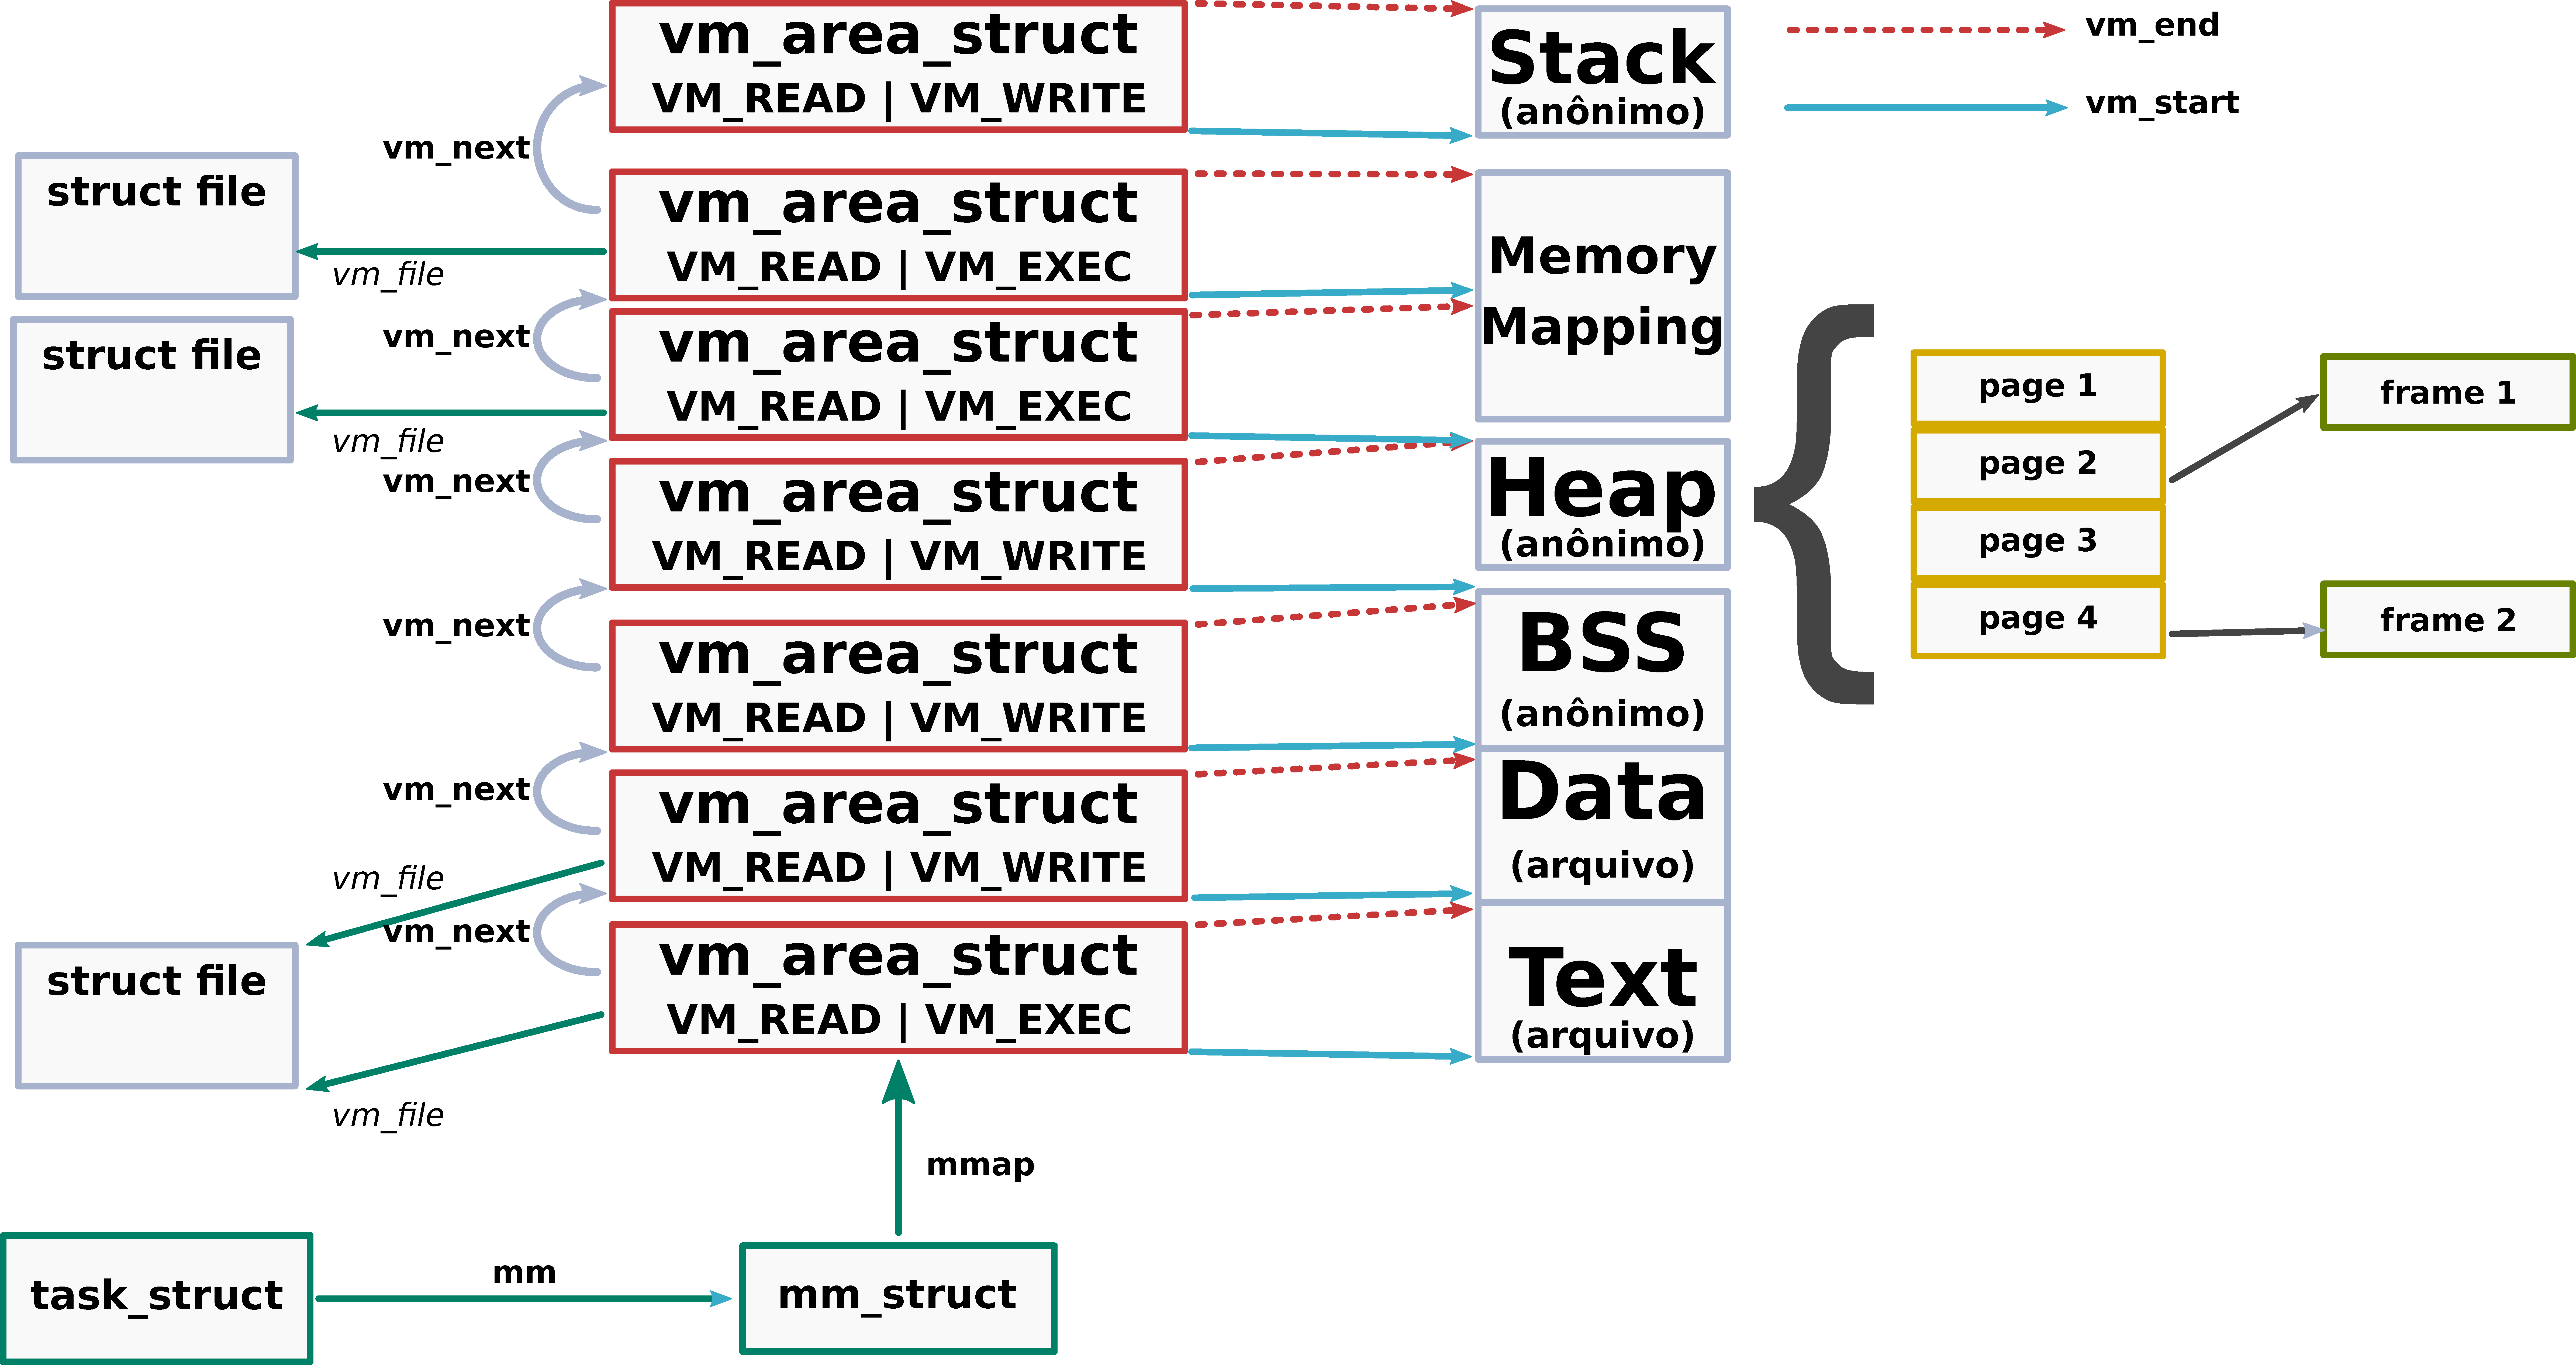
\includegraphics[width=\textwidth]{kernel_manages_memory}
	\caption[Visão interna do gerenciamento da memória]{Visão interna do gerenciamento da memória~\citep{kernel_manage_mem}}
  \label{fig:kernel_manages_memory}
\end{figure}

Observando a Figura~\ref{fig:kernel_manages_memory} sob a ótica
da implementação, temos as estruturas de dados usadas pelo Linux e
suas ligações. No Kernel, a estrutura responsável por manter todas as
informações do processo (i.e., PCB) chama-se \texttt{task\_struct}. Ela tem um
ponteiro para outra estrutura de dados chamada de \texttt{mm\_struct}, que
mantém uma lista ligada para estruturas do tipo \texttt{vm\_area\_struct} (ou
\boldAndIndex{virtual memory area --- VMA}). Uma VMA consiste em um intervalo de
endereços virtuais contíguos e sem sobreposição; elas também possuem algumas
\textit{flags} de controle de acesso associadas. A informação se a VMA é
anônima ou não vem do campo \texttt{vm\_file} (se ele estiver vazio, então a
área é anônima). Repare na figura que cada segmento corresponde a uma VMA; a
única exceção são os segmentos de mapeamento de memória, que podem ter mais de um
VMA. Lembre-se que a VAS é dividida em páginas, por isso o tamanho de uma VMA
deve ser múltiplo do tamanho de uma página. De forma geral, a VMA, em conjunto com a
tabela de páginas, orquestra o gerenciamento do programa na memória no Linux.

%\begin{figure}[!h]
%  \centering
%  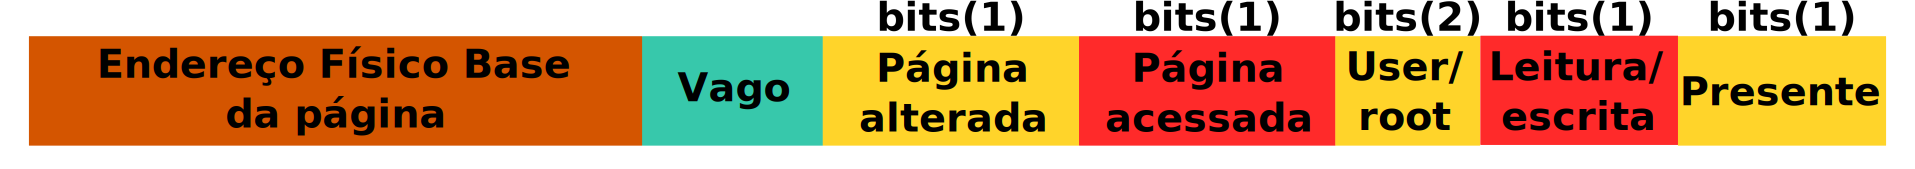
\includegraphics[width=\textwidth]{pte}
%  \caption{Entrada da tabela de páginas}
%  \label{fig:pte}
%\end{figure}
%
%Toda vez que um acesso à memória é feito, a tabela de páginas do processo é
%consultada. Cada entrada dessa tabela é descrita por uma série de metadados
%que descreve a região de memória e recebe o nome de
%\boldAndIndex{entrada da tabela de páginas} (\textit{Page Table Entry}) ou
%simplesmente PTE. A Figura~\ref{fig:pte} ilustra como a entrada pode ser
%representada\footnote{Cada arquitetura implementa a PTE à sua maneira.}. Sem
%entrar em detalhes referentes aos campos (a figura é autoexplicativa), podemos
%concluir que uma página virtual é a unidade mínima de proteção da memória, por que
%todos os bytes dela compartilham os bits User/Root e Leitura/Escrita.

\begin{figure}[!h]
  \centering
  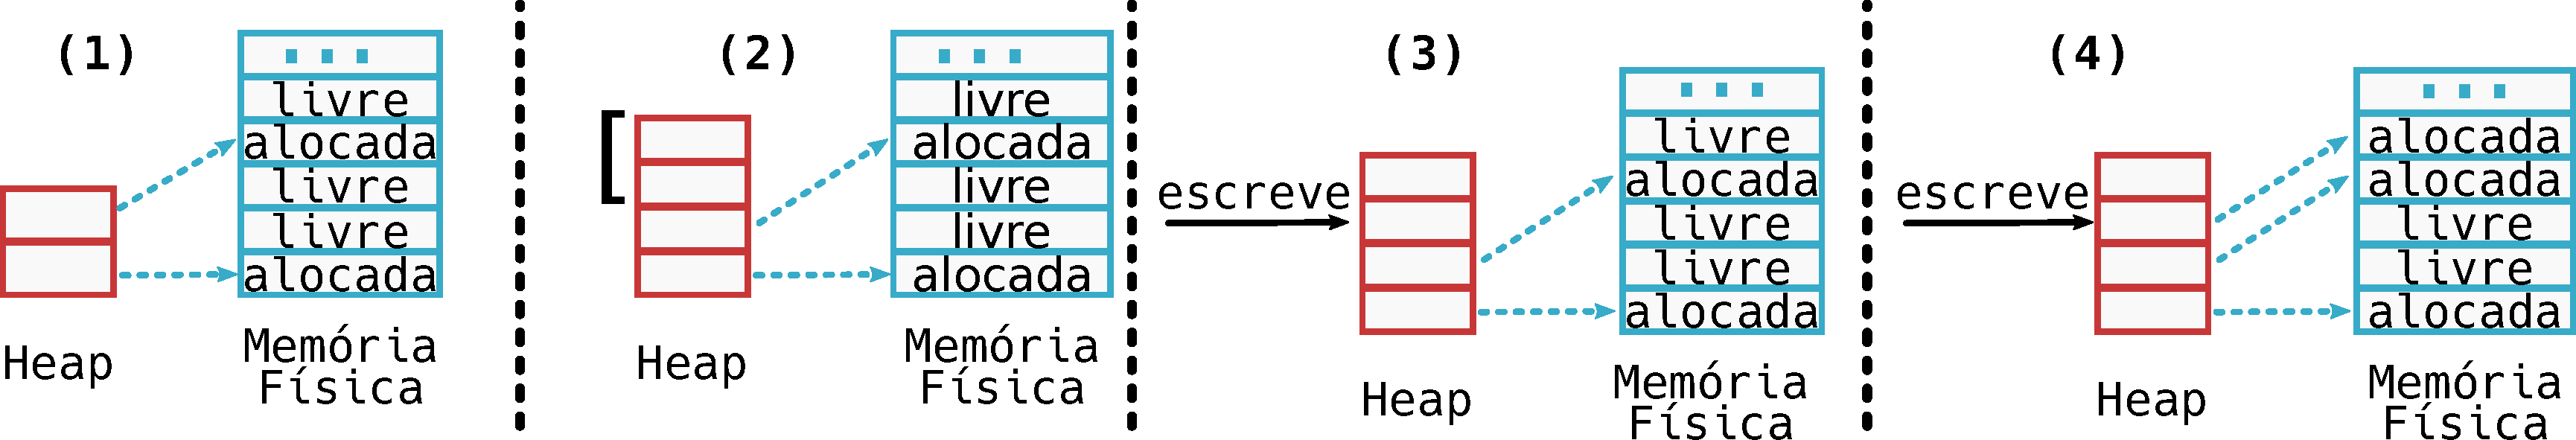
\includegraphics[width=\textwidth]{malloc}
  \caption[Passos envolvidos na alocação de memória com \texttt{malloc()}]{Passos envolvidos na alocação de memória com \texttt{malloc()} (imagem baseada em \cite{anatomy_program_mem})}
  \label{fig:malloc_linux}
\end{figure}

Por fim, para exemplificar como esses mecanismos estão relacionados do kernel ao
espaço do usuário, veja a Figura~\ref{fig:malloc_linux}. Na figura, temos um programa com
algumas páginas já mapeadas para uma memória física. A aplicação decide alocar
mais memória por meio da função \texttt{malloc()}, e por sua vez, uma chamada
para \texttt{brk()} é feita. O kernel atualiza o VMA do \textit{heap} com o
tamanho solicitado e fornece o ponteiro para a aplicação. Na prática, nenhum
endereço físico foi alocado e, enquanto o programa não acessar a região alocada,
nenhum \emph{frame} é criado. Na primeira tentativa de acesso, ocorre uma falha
de página e a função \texttt{do\_page\_fault()} é chamada. Se o processo
atender à permissões indicadas na PTE, então o kernel aloca e associa o
\emph{frame} à página.

\section{Chamadas de Sistema}
% TODO: Fazer a distinção entre user space e kernel space
% TODO: Falar do SYSCALL e VMSYSCALL - Atualizar o Dune

\citet{silberschatz} apresenta diversas perspectivas sobre SOs. Dentre elas,
destaca-se a ideia de que um SO fornece serviços para tornar as tarefas de
programação mais simples para os desenvolvedores. Partindo de tal concepção,
podemos notar os seguintes serviços: controle sobre a execução de um programa,
operações de E/S, manipulação de sistemas de arquivos, comunicação via rede,
detecção de erros, alocação de recursos, dentre outros. Dada a vasta quantidade
de serviços oferecidos, levantamos a questão de qual mecanismo é utilizado pelo
SO para fornecer acesso a eles? A resposta é simples: chamadas de
sistema (também conhecidas por \emph{system calls} ou \emph{syscalls}).

Uma \boldAndIndex{chamada de sistema}
consiste em uma operação de API de baixo nível que permite que uma aplicação executando no
espaço de usuário (\emph{user space}) faça uma requisição para o SO. Por sua
vez, esse pedido é rigorosamente validado pelo SO, que pode executar a operação
até o fim, devolvendo o que a aplicação solicitou, ou pode se negar a
executá-la, caso encontre algum impedimento. Na prática, esse tipo de operação
consiste em uma simples chamada de função que é tratada pelo SO. Normalmente,
cada \emph{syscall} tem um número associado a si, através do qual o SO consulta
uma tabela que identifica a função que deve ser executada. Além disso, passar
parâmetros para esse tipo de função pode depender da arquitetura e de outros
detalhes. Para tentar esconder toda a complexidade por trás desse tipo de
operação, muitas vezes são escritas bibliotecas que encapsulam esse tipo de
chamada. O exemplo mais emblemático é a \emph{libc} que oculta vários detalhes
de baixo nível, como a leitura e escrita de um arquivo.

\begin{figure}[!h]
  \centering
  \includegraphics[width=0.5\textwidth]{userspace_to_kernel} 
  \caption{Execução do user space até o kernel space}
  \label{fig:userspace_kernelspace}
\end{figure}

Para ilustrar como esse conceito funciona na prática, veja a
Figura~\ref{fig:userspace_kernelspace}. Nela, um programa pede o
seu PID para o SO (exemplo baseado em \cite{syscallex}). O programa executado
está na memória e tem o seu \emph{Address Space} devidamente inicializado;
ao invocar a função \texttt{getpid()}, o seu fluxo de execução é levado para a
\emph{libc}. Por sua vez, a \emph{libc} faz algumas operações, tal como alocar
espaço na memória para fazer cache do PID. Quando a \emph{libc} está pronta,
ela finalmente faz a chamada para o sistema. Note que nessa etapa ocorre uma
mudança de um modo de execução menos privilegiado (\emph{ring 3}) para um modo
privilegiado (\emph{ring 0}). Nesse momento, o SO tem total controle sobre o
pedido feito e faz a verificação dos parâmetros e permissões. Se tudo correr
bem, o SO se encarrega de copiar a informação pós-processada do espaço do
Kernel para o espaço do usuário. Por fim, a \emph{libc} salva o valor do seu
cache, evitando a necessidade do SO intervir no futuro e a aplicação finalmente
recebe o seu PID.

\section{Troca de Contexto}

Em um SO de propósito geral, um processo executa por um intervalo de tempo;
quando esse tempo acaba outro processo é inserido na CPU, esse procedimento
ocorre na escala das centenas de processos. A troca tem início quando uma
interrupção vinda do hardware ocorre, seja ela porque o tempo de CPU do
processo terminou ou por qualquer outro motivo. O primeiro passo necessário
consiste em salvar o estado do processo em execução e, em seguida, carregar o
estado do novo processo na CPU. Repare que o tempo gasto na troca de processo
não produz nenhum trabalho útil, ou seja, é um
\textit{overhead}~\citep{silberschatz}.

Na prática, a troca de contexto é bem mais complexa. Por exemplo, vamos olhar
de perto e de forma breve a troca de contexto no GNU/Linux em uma arquitetura
x86.  Primeiramente, todos os processos precisam compartilhar os registradores
da CPU. Por esse motivo, o kernel deve assegurar que todos os registradores
sejam carregados com os valores de quando o processo foi suspenso. O conjunto
de todos os dados dos registradores que devem ser carregados recebe o nome de
\boldAndIndex{contexto de hardware}~\citep{entendendo_kernel}, que pode ser
visto como um subconjunto do contexto do processo. No Linux, o contexto de
hardware é armazenado na própria estrutura do processo, enquanto as demais
partes são salvas em uma interna pilha do kernel. Toda troca de processo
precisa armazenar o contexto de hardware, por isso a \texttt{task\_struct}
inclui um campo chamado \texttt{thread\_struct}, que armazena o contexto do
hardware (dependente da arquitetura de hardware).

Para realizar a troca de processos, o Kernel Linux realiza duas
operações~\citep{entendendo_kernel}: (1) Instala o novo espaço de endereço e
(2) Muda a pilha do domínio do Kernel e o contexto de hardware

A operação de troca é extremamente dependente da arquitetura de hardware, pois
precisa ser executada de forma rápida e, por isso, o Linux tenta tirar proveito
de todo recurso disponibilizado pela CPU\footnote{Note que é preciso levar em
consideração os registradores que lidam com pontos flutuantes, o que faz a troca
de contexto ainda mais pesada}.

% Falar de PCID?
\section{Descritores de Arquivo}

Normalmente, quando um processo deseja ler ou escrever um dado em um arquivo,
ele precisa passar por algumas camadas. O processo interage com o
\boldAndIndex{sistema de arquivos}, que é responsável por fornecer um mecanismo
simplificado para o processo localizar, escrever e recuperar dados. Por sua
vez, os sistemas de arquivos atuam com outras camadas responsáveis por manter a
organização e meta-dados dos aquivos. Por fim, as operações de alto nível são
convertidas para instruções de baixo nível passadas para os discos que de fato
realizam as operações solicitadas.

Em GNU/Linux e outros sistemas POSIX, existe uma estrutura de dados utilizada
para controlar o bloco de dados em disco e que é usada para leitura ou escrita,
o \boldAndIndex{inode}. Um inode contém diversas informações, dentre elas:
permissão, datas, dono do arquivo, tamanho, dentre outros. Quando um arquivo é
criado, uma estrutura de dados como o inode é criada e então o arquivo é salvo.

Quando um processo abre um arquivo, ele faz uma chamada para \texttt{open()},
acionando o sistema de arquivos para encontrar o arquivo solicitado.
Para isso, \texttt{open()} primeiro procura em uma \boldAndIndex{tabela global
de arquivos} para verificar se o arquivo solicitado já está aberto. Se o
arquivo estiver presente na tabela global, uma nova entrada em uma
\boldAndIndex{tabela local de arquivos dos processos} é feita e nela é
armazenada uma nova entrada com a posição referente ao arquivo na tabela
global. A tabela global é atualizada com a informação de que um novo processo
abriu o arquivo (basicamente, um contador é incrementado para representar a
informação). Por outro lado, se não existe uma entrada para o arquivo solicitado
na tabela global, ele é carregado e a tabela global atualizada. A
Figura~\ref{fig:descritores} ilustra a operação descrita.
 
\begin{figure}[!h]
  \centering
  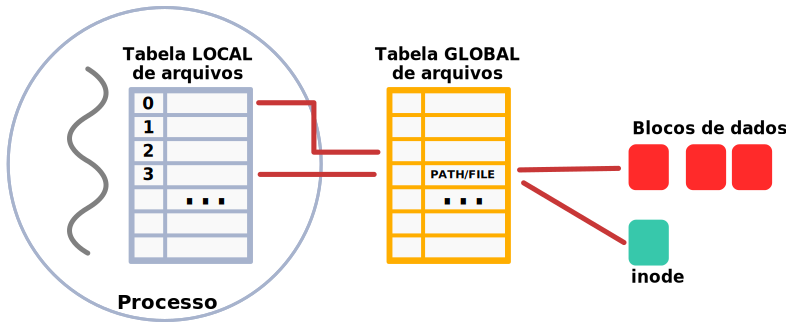
\includegraphics[width=.70\textwidth]{descritores} 
  \caption{Tabela local e global de arquivos}
  \label{fig:descritores} 
\end{figure}

Quando um arquivo é aberto por meio da função \texttt{open()}, ela devolve um
número chamado de \boldAndIndex{descritor de arquivo (file descriptor --- fd)},
que nada mais é do que a posição da entrada na tabela local de processos.
Quando o processo fecha um arquivo, a entrada na tabela local é removida e o
contador de processos presente na tabela global é decrementado. Quando o
contador zera, o bloco de dados referente ao arquivo aberto é finalmente
atualizado.

\section{Modelos de Programação}

Além da manipulação de dispositivos de hardware, os SOs fornecem vários
recursos adicionais para o espaço de usuário, tal qual \emph{file locking} e
primitivas de segurança. Para fazer uso de tais recursos, a aplicação precisa
ser capaz de acessá-los por meio de um modelo de programação coerente, i.e., um
conjunto bem estabelecido de abstrações interligadas. Um dado SO implementa um
dado modelo de programação através de uma API própria. Por exemplo, tanto o
GNU/Linux quanto Windows fornecem diferentes APIs de \emph{threading}
(\emph{pthreads} e \emph{WindowsThreads}), mas ambos correspondem ao modelo de
programação de paralelismo.

Atualmente, a maioria dos SOs dá suporte a um grande número de modelos de
programação e suas respectivas APIs. Contudo, as aplicações mudam ao longo dos
anos e criam demandas para melhorias em áreas como camadas de segurança, opções
de otimização e simplificação de código; esses aspectos são problemas reais.
Consequentemente, propostas para expandir as abstrações de processos visando
introduzir novos modelos de programação são recorrentes e representam uma
interessante área para inovações.

%TODO: Mudar esse nome para algo melhor
\section{Aspectos de Implementação}

As abstrações de processos são o ponto central no projeto de um SO moderno,
mapeando outras abstrações para ele. Assim, outros serviços são oferecidos pelo
SO com a intenção de fornecer os mecanismos necessários para orquestrar todas
as operações dos processos (p.ex., escalonador e gerenciamento de memória). Toda
estrutura necessária para gerir processos tem o lado negativo de utilizar CPU
(\emph{overhead}); para tentar mitigar essa situação, os SOs empregam um vasto
número de otimizações de hardware e software.

Mudanças em uma abstração de processos normalmente têm impactos no desempenho e
as consequências podem variar de acordo com a proposta de modificação. Por
exemplo, uma verificação adicional em uma camada pode elevar a sobrecarga no
sistema devido a uma nova característica implementada. Contudo, enquanto
extensões de processos podem degradar o desempenho, elas também podem trazer
benefícios de desempenho explorando alguma característica do hardware.

\section{Gerenciamento de Recursos}

Toda aplicação em execução em um SO consome recursos do sistema.
Frequentemente, elas realizam boa parte do trabalho no espaço de usuário, o que
requer pouca intervenção do SO. Por exemplo, uma aplicação que faz cálculos
complexos não precisa de muita intervenção do SO. Contudo, existe uma grande
quantidade de software que demanda significativa participação do SO para
atingir os seus objetivos, estendendo assim o seu consumo de recursos para o
sistema. Por exemplo, uma aplicação que utiliza recursos de rede tem várias
partes das suas atividades conduzidas pelo SO quando um pacote chega.

Esse cenário no qual a aplicação solicita que o SO execute algo em seu favor,
faz com que o consumo de recursos por parte da aplicação atravesse do espaço de
usuário para o espaço do kernel. Essa situação pode gerar problemas devido ao
controle indireto e descontrolado do uso de recursos; ataques de negação de serviço
(\emph{Denial-of-service}) representam um exemplo da vida real que eleva o
consumo do uso de recursos por parte do SO.

\section{Outros Conceitos Indiretamente Relacionados a Abstração de Processos}

Nesta seção, apresentaremos o tópico de \emph{device drivers} e virtualização.
Esses são temas indiretamente relacionados às abstrações de processos e que são
tratados aqui para auxiliar o leitor na leitura dos próximos capítulos. Vale
observar que esses conceitos representam poderosas ferramentas para expandir as
abstrações de processos.

\subsection{Device Drivers}
\label{sec:dd}

Um SO é repleto de elementos que buscam manipular e ocultar a complexidade de
lidar com o hardware, portanto, esse é um dos motivos pelos quais esse tipo de
software é consideravelmente grande e complicado. Para tornar esse cenário
ainda mais desafiador, é preciso levar em consideração que um SO deve fornecer
suporte para uma infinidade de dispositivos. A forma como os \emph{drivers}
interagem com o Kernel deve ser projetada com muito cuidado visando reduzir a
complexidade e o acoplamento. O design adotado na maioria dos SOs é uma
abordagem flexível na qual o código para um dispositivo é mantido isolado em um
\emph{driver}.

O isolamento fornecido por um \emph{device driver} é interessante, uma vez que
ele fornece um mecanismo e não uma política \citep{ddbook}. Entenda por
mecanismo a capacidade que deve ser fornecida e, por política, a forma com
que a capacidade deve ser usada. Esse separação é interessante pois limita o
que um \emph{driver} deve fazer e, por sua vez, simplifica a implementação. Um
exemplo disso é o \emph{Direct Rendering Managemente} do Linux, que
fornece várias capacidades, dentre elas, a operação de trocar
\emph{framebuffers} primários e secundários; contudo, é a aplicação que deve
controlar tal operação.

Por fim, é interessante ressaltar que alguns sistemas fornecem a ideia de
\boldAndIndex{módulos carregáveis} (\textbf{loadable modules}), que significa
que, em tempo de execução, é possível carregar um novo \emph{device driver}. Esse
tipo de funcionalidade torna o SO mais leve e configurável. Os módulos
são extremamente flexíveis do ponto de vista da implementação uma vez que são
um código separado do núcleo do SO e respeitam a interface definida pelo mesmo.

\subsection{Virtualização}
\label{sec:virtualizacao}

% TODO: Eu acho que faltou introduzir alguns dos termos básicos logo no início
% contar um pouco como funciona e acertar a fluídez do texto
% TODO: Falar brevemente do KVM - Atualizar o Dune

A ideia de oferecer a abstração de máquinas virtuais dentro de uma mesma
máquina é um aspiração de longa data, como o emblemático trabalho de Popek e
Goldberg demonstra~\citep{popek}. Ele foi publicado em 1974 e indicava os
requisitos necessários para que a terceira geração de processadores fornecessem
virtualização completa. Naquele período, se tinha noção de algumas das vantagens
que a virtualização por software e hardware poderia entregar. Dentre os
inúmeros benefícios da virtualização, destacam-se a possibilidade de executar
aplicações legadas de um SO antigo, recursos que facilitam o processo de
desenvolvimento de software, serviços de nuvem, \emph{checkpoints}, migração de
processos, isolamento, dentre outras.

O elemento central da virtualização é o \boldAndIndex{hypervisor} (também
conhecido como \boldAndIndex{Virtual Machine Monitor (VMM)}), que é responsável por
criar a ilusão de múltiplas máquinas em um mesmo hardware
físico~\citep{tanenbaum}. Essas máquinas virtuais executam sobre o mesmo hardware
e tem a capacidade de executar diferentes SOs. Existe a ideia de máquina
convidada (\boldAndIndex{guest}) e máquina hóspede (\boldAndIndex{host}). A
primeira refere-se ao SO que está executando sobre o VMM e a segunda refere-se
à máquina que está executando sobre o hardware com privilégios.

Um dos objetivos da virtualização consiste em permitir que um SO inicialize
como se estivesse em uma máquina real. Para que isso seja possível, é preciso
emular o hardware de forma que o \emph{guest} não perceba que está em um
ambiente simulado e, ao mesmo tempo, de forma
eficiente. Em 1974, \citet{popek} sugeriram alguns requisitos para que os
hardwares pudessem oferecer suporte completo para virtualização,
amplamente implementados nos processadores modernos. Os autores também
destacam três dimensões que devem ser consideradas para fornecer a
virtualização completa no nível dos processadores: segurança, fidelidade e
eficiência.

No que tange o assunto segurança, o VMM deve ter total controle sobre os
recursos virtualizados. Uma opção é utilizar um interpretador que intercepta
cada instrução e realiza exatamente o que a instrução precisa. Algumas
instruções podem ser executadas diretamente, mas outras não. Por exemplo, não
deve ser possível para a máquina \emph{guest} desativar as interrupções de toda
a máquina \citep{tanenbaum}. Para contornar tal situação, o SO \emph{guest}
deve ter a ilusão de que as interrupções estão desativadas.

Do ponto de vista da fidelidade, o comportamento do programa em execução na
máquina virtual deve ser idêntico ao seu comportamento se ele estivesse executando
diretamente no hardware. Na prática, existem várias complicações associadas a
esse requisito que levam à categorização das instruções utilizadas pela CPU em
três grupos de diferentes:

\begin{itemize}
  \item \boldAndIndex{Instruções sensíveis}: CPUs que fornecem \emph{user mode} e
        \emph{kernel mode} apresentam instruções comuns para ambos os modos de
        operação, mas que têm comportamentos diferentes dependendo de cada modo
        de operação no qual a instrução é executada;
  \item \boldAndIndex{Instruções privilegiadas}: São instruções que geram uma
        \emph{trap} quando executadas no modo usuário, mas que não geram
        \emph{trap} em modo Kernel;
  \item \boldAndIndex{Instruções de controle de fluxo sensíveis}: São aquelas que
        tentam mudar a configuração de algum recurso do sistema.
\end{itemize}

Se um programa tentar fazer algo em modo usuário que não deveria ser capaz de
fazer, o hardware deve capturar essa ação; em outras palavras, Popek e Goldberg
mostraram que uma máquina é virtualizável se o conjunto de instruções sensíveis
é um subconjunto das instruções privilegiadas. Apesar de parecer um conceito
simples, foram necessários vários anos para que as CPUs incorporassem tais funcionalidades
e assim oferecessem um adequado suporte de hardware para a virtualização.

O uso de técnicas de virtualização já era conhecido muito antes de 1998,
contudo nenhuma das abordagens utilizadas naquele período tinha total suporte
para a virtualização em hardware que atendesse os três tipos de instruções
indicado por \citet{popek}. O suporte completo para a virtualização em hardware
foi resolvido apenas em 2005 pela Intel~\citep{uhlig} com uma tecnologia
chamada \textbf{Virtualization Technology (VT-x\index{VT-x})}. A AMD tem uma
solução parecida chamada \boldAndIndex{Secure Virtual Machine (SVM)}. A ideia
básica é criar um invólucro no qual a máquina virtual pode executar um SO
\emph{guest}.  O SO continua em execução até que provoque uma \emph{trap} que
faça o VMM ter que lidar com a situação. O conjunto de instruções que provocam
uma \emph{trap} é controlado por um conjunto de bits ao qual o VMM tem acesso.
A extensão VT-x torna possível a execução clássica de uma máquina virtual
baseada em interrupção-e-emulação~\citep{tanenbaum}.

Do ponto de vista da eficiência, a virtualização deve fazer com que a maior
parte do código executado pelo SO \emph{guest} não sofra interferência do VMM.
Uma das abordagens utilizadas antes de se ter o hardware de virtualização foi a
adoção de técnicas na qual o \textit{hypervisor} interceptava as instruções e
as reescrevia em tempo de execução com uma sequência de código considerada
segura. Esse mecanismo permitia substituir instruções sensíveis, mas não
privilegiadas. Tal técnica ficou conhecida como \boldAndIndex{tradução binária}
e demostrou-se extremamente eficiente devido ao seu sofisticado mecanismo de
\emph{cache}.

% TODO: Falar dos tipos de hypervisor
%FIGURA X

\subsubsection{A Tecnologia VT-x}
\label{sec:vtx}

\citet{uhlig} apresentaram a tecnologia de virtualização adotada pela Intel para
fornecer a virtualização completa no nível do processador. A
Figura~\ref{fig:vt-x_flow} ilustra os elementos que compõem a tecnologia VT-x e a
forma como eles interagem. Dentre as inovações apresentadas, dois novos modos
de operação introduzidos nas CPUs merecem destaque: \emph{VMX non-root} e
\emph{VMX root}.

O \boldAndIndex{VMX non-root} é o modo de operação no qual a máquina
\emph{guest} executa, enquanto o \boldAndIndex{VMX root} é o modo de operação utilizado
pelo VMM. É interessante observar que os dois modos têm suporte para os quatro
níveis de privilégios fornecidos pelos processadores Intel; isto permite que a
máquina \emph{guest}, ao tentar executar uma instrução privilegiada em algum
desses níveis, forneça informações para o VMM. Os software em execução como
\emph{VMX non-root} (p.ex., uma máquina com Debian) pode tentar acessar um dos
modos privilegiados, contudo o modo \emph{non-root} não tem privilégios reais
para executar instruções que exigem permissões maiores que a sua; nesses casos,
o VMM entra em ação para intermediar a situação.

\begin{figure}[!h]
  \centering
  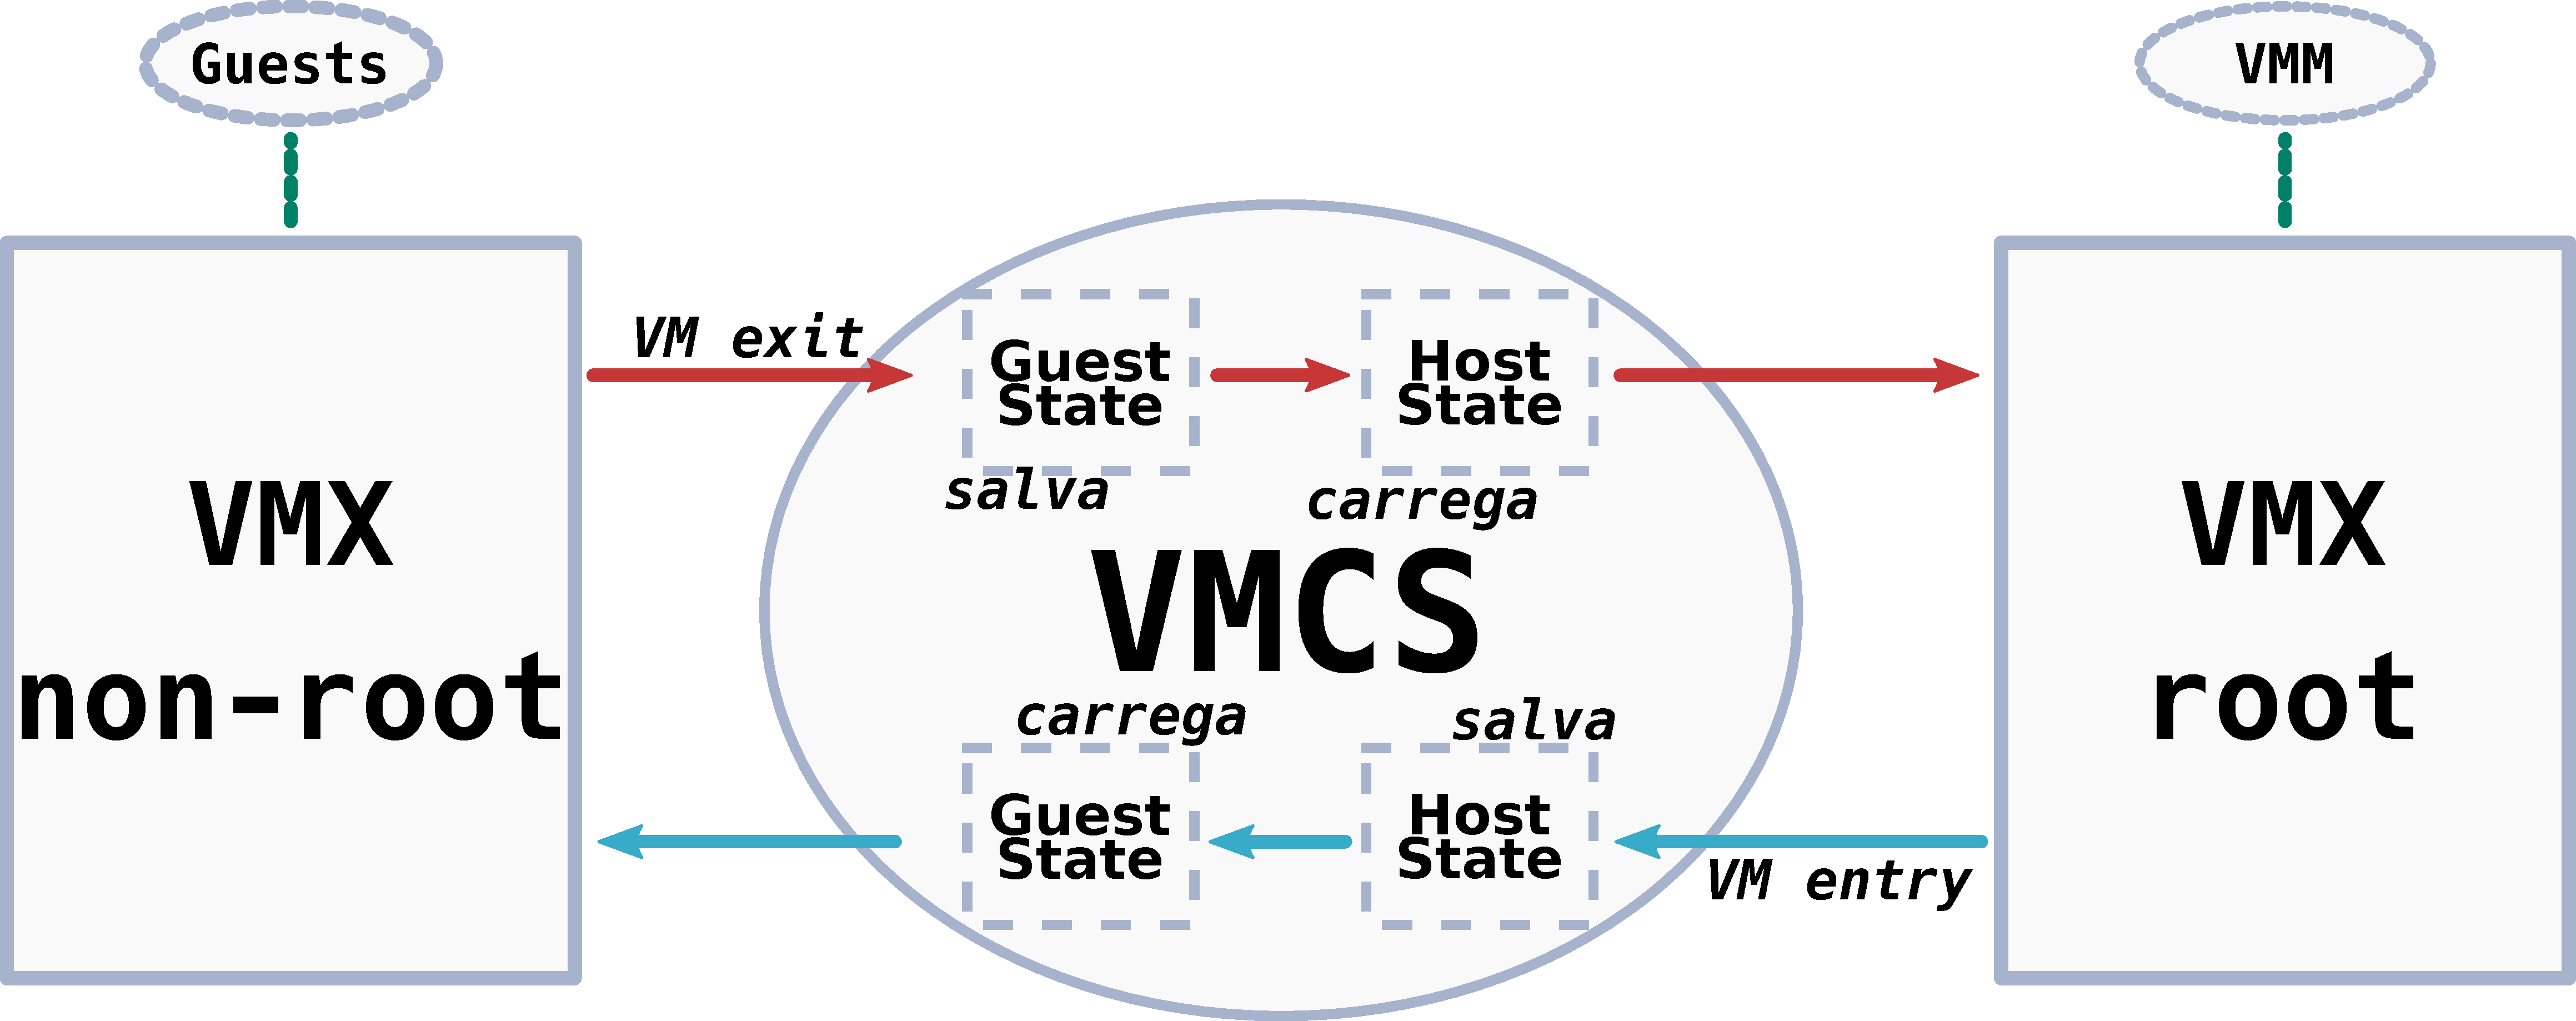
\includegraphics[width=0.7\textwidth]{vt-x_flow} 
  \caption{Fluxo do comportamento da tecnologia VT-x}
  \label{fig:vt-x_flow}
\end{figure}

A Figura~\ref{fig:vt-x_flow} mostra as transições \boldAndIndex{VM exit} e
\boldAndIndex{VM entry}. A transição \emph{VM exit} ocorre quando o controle é
transferido do \emph{guest} para o VMM, fazendo com que o estado da máquina
\emph{guest} seja salvo e o estado do \emph{host} seja carregado para que o VMM
decida como tratar a interrupção. No sentido oposto, ocorre a transição
\emph{VM entry}: nesse caso, o VMM transfere o controle para a máquina
\emph{guest}, salvando o estado do \emph{host} e carregando o estado
anterior do \emph{guest}. Todas as informações referentes à virtualização são
mantidas em uma estrutura de dados chamada \boldAndIndex{virtual-machine
control structure (VMCS)} que tem por função gerenciar as transições entre a
\emph{VM entry} e \emph{VM exit}.

Na prática as CPUs Intel fornecem diversas instruções para utilizar o VT-x. Em
especial, o \texttt{VMCALL} faz com que \emph{VM Exit} ocorra
incondicionalmente, transferindo o controle para o VMM; por sua vez, o VMM
decide o que fazer. Para a melhor compreensão do conteúdo dos próximos
capítulos desta dissertação, destacamos apenas um pequeno subgrupos de
instruções que normalmente são expostas para as máquinas \emph{guest} por meio
do VT-x de forma segura e isolada, são elas~\citep{intelmanual}:

\begin{description}
	\item [\textbf{Exceções}:] São tipos especiais de transferência de
controle; elas alteram o fluxo normal de execução do programa para atender
algum evento externo ou reportar erros para situações excepcionais. Em resumo,
exceções manipulam condições detectadas pelo processador no decorrer da
execução de uma instrução;
		\begin{itemize}
			\item \texttt{LIDT}: Carrega o valor que indica a localização de um
endereço base para ser carregado no registrador que mantém a referência para a
tabela global de descritores ou a tabela de interrupções;
			\item \texttt{LTR}: Carrega um segmento específico que aponta para o
segmento de estado de um processo. Essa instrução só pode ser executada em modo
privilegiado;
			\item \texttt{IRET}: Devolve o controle para um programa ou procedimentos
após a manipulação de uma exceção ou interrupção;
			\item \texttt{STI}: Ajusta a \emph{flag} \texttt{IF} em um registrador
\texttt{EFLAGS}, depois de ajustado, o processador começa a responder a
interrupções externas;
			\item \texttt{CLI}: Limpa a \emph{flag} de interrupção.
		\end{itemize}
  \item [\textbf{Memória Virtual}:]
Máquinas virtuais precisam lidar com o gerenciamento da memória, para isso,
elas precisam fazer uso de instruções de manipulação da memória em conjunto com
um recurso chamado de \emph{Extended Page Tables (EPT)} -- discutiremos a seguir;
		\begin{itemize}
			\item \texttt{MOV CRn}: Esse tipo de instrução é usada para manipular
bits dos registradores, no contexto das memórias virtuais, os registradores CR2
e CR3 são dois importantes elementos. O primeiro é usado para identificar
faltas de página e o segundo contém o endereço físico base de uma hierarquia de
página em conjunto com duas \emph{flags} de controle;
			\item \texttt{INVLPG}: Invalida entradas na TLB;
			\item \texttt{INVPCID}: Invalida entrada nas TLBs e \emph{caches} de
página.
		\end{itemize}
	\item [\textbf{Modos Privilegiados}:] Operações realizadas em modos
privilégiados.
		\begin{itemize}
			\item \texttt{SYSCALL}: Chamada rápida para o modo privilegiado;
			\item \texttt{SYSRET}: Trabalha em conjunto com a instrução
\texttt{SYSCALL} devolvendo a execução do SO para o modo de usuário;
			\item \texttt{SYSEXIT}: Devolve de forma rápida a execução para a
aplicação no espaço de usuário.
		\end{itemize}
\end{description}

Por fim, o VT-x trabalha com uma tecnologia chamada de Tabelas de Páginas
Estendidas (EPT) que é uma extensão feita sobre as MMUs. O EPT é um mecanismo
de paginação aninhada que trata cada endereço físico da máquina \emph{guest}
como um endereço virtual na máquina \emph{host}, inserindo multiníveis na
tabela de páginas da máquina \emph{host}. Note que toda a manipulação é feita
com o auxílio do hardware, o que torna todo o processo de tradução eficiente.

\section{Considerações Finais}

Neste capítulos, buscamos apresentar os diversos temas ligados direta e
indiretamente às abstrações de processos com o objetivo de tornar a leitura
desta dissertação mais simples. No próximo capítulo, apresentaremos diversos
trabalhos na qual acreditamos representar o estado da arte nas abstrações de
processos e que ainda não atingiram os SOs de produção.

